\documentclass[10pt]{beamer}
\usetheme{Malmoe}
\colorlet{beamer@blendedblue}{green!40!black}
\setbeamertemplate{navigation symbols}{}
\newcommand*\oldmacro{}%
\let\oldmacro\insertshorttitle%
\renewcommand*\insertshorttitle{%
\oldmacro\hfill%
\insertframenumber\,/\,\inserttotalframenumber}

\usepackage{caption}
\usepackage{hyperref}
\usepackage[makeroom]{cancel}
\usepackage{ amssymb }
\usepackage{appendixnumberbeamer}
%\usepackage{tikz-feynman}
\usepackage{graphicx}
\begin{document}
\title{Search for Flavor Changing Neutral Currents in Top Quark Decays}
\subtitle{$t \rightarrow q \gamma$}
\author[Barkeloo, Comprehensive Exam]{Jason Barkeloo}

\titlegraphic{
\includegraphics[width=4cm]{../ATLAS-Logo-Ref-RGB.png}\hspace*{2.75cm}~%
   
\includegraphics[width=4cm]{../uo_logo_green_on_white_2.jpg}
}

\date{November 30, 2017}
\frame{\titlepage}
\frame{\frametitle{Table of Contents}\tableofcontents[hidesubsections]}
\section{The Standard Model and the Top Quark}
%\frame{\frametitle{Table of Contents}\tableofcontents[currentsection,hideothersubsections]}
%%%%%%%%%%%%%%%%%%%%%%%%%%%%%%%%%%%%%%%%%%%%%%%%%%%%%%%%%
\subsection{The Standard Model}

%%%%%%%%%%%%%%%%
\frame{\frametitle{The Standard Model}
\begin{figure}
	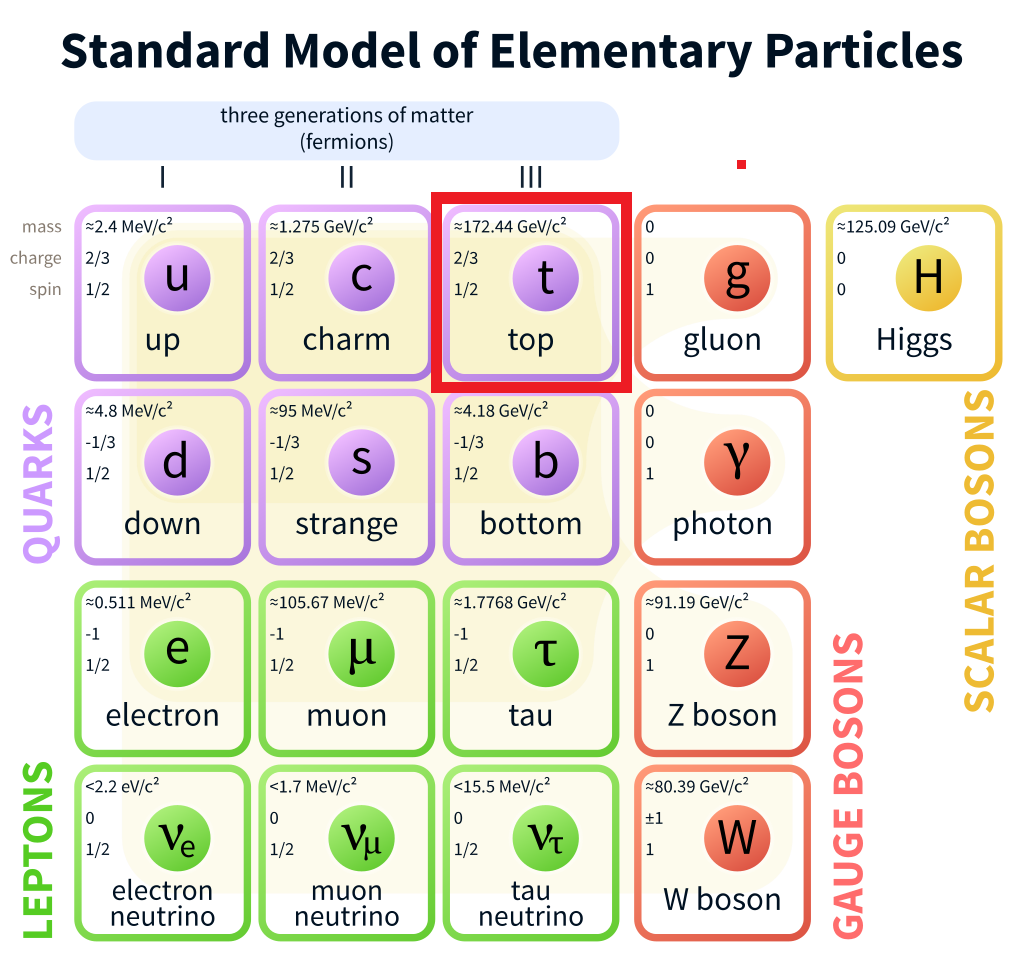
\includegraphics[width=4.8cm]{../../ThesisImages/SMParticles.png}
	\captionof{figure}{\href{https://en.wikipedia.org/wiki/Standard_Model}{List of standard model particles}}
\end{figure}
\begin{itemize}
\item Our current theory that attempts to explain everything
	\begin{itemize}
	\item Experimentally precise and well behaved
	\item Very few exceptions (i.e. Neutrino Mass, Matter-Antimatter Asymmetry, Dark Matter Abundance)
	\end{itemize}
	\vspace{\baselineskip}
\end{itemize}
}

\subsection{The Top Quark}

%%%%%%%%%%%%%%%%%%%%
\frame{\frametitle{The Top Quark}
\begin{itemize}
\item Heaviest fundamental particle, $172.5 GeV$
\item Lifetime $5x10^{-25}s$, decays before hadronization
	\begin{itemize}
	\item Allows us to study the decay of a single quark
	\end{itemize}
\end{itemize}
\begin{figure}
	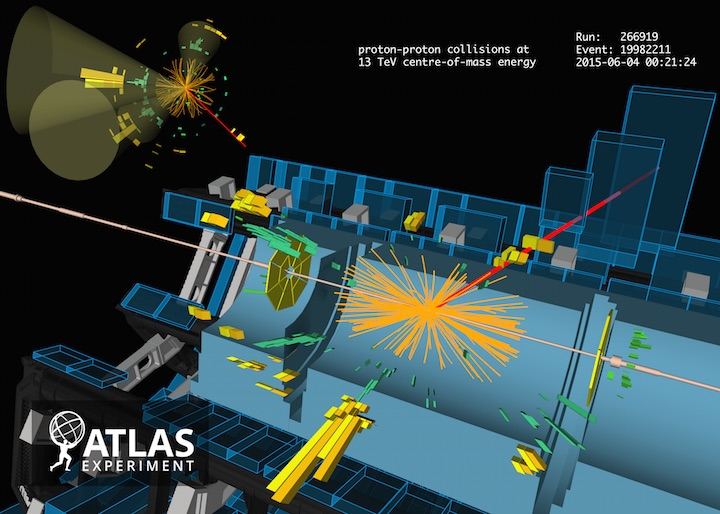
\includegraphics[height=0.5\textheight]{../../ThesisImages/ttbarevent.png}
	\captionof{figure}{$t\bar{t}$ event in the ATLAS detector}
\end{figure}
}

\frame{\frametitle{Top Quark Pair Production}
\begin{itemize}
\item Leading order processes for top quark production
	\begin{itemize}
	\item Quark-antiquark annihilation $\approx 10\%$
	\item Gluon-gluon fusion $\approx 90\%$
	\end{itemize}
\end{itemize}
\centering

	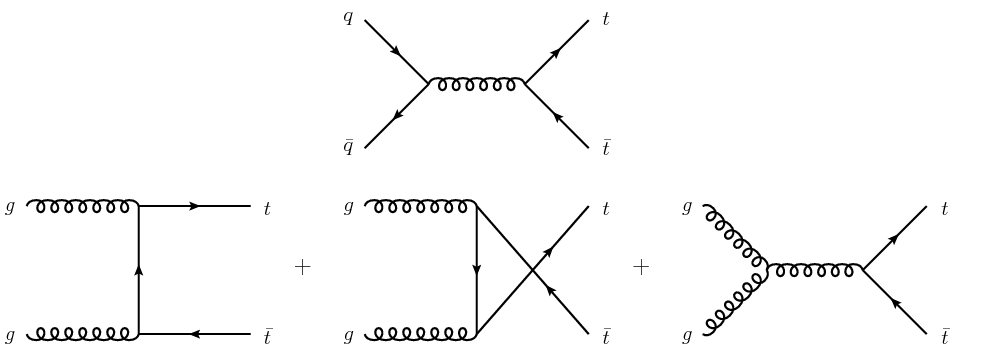
\includegraphics[height=0.5\textheight]{../../ThesisImages/LOPairProdDiags.png}
	\captionof{figure}{Leading order $t\bar{t}$ diagrams}
}

\frame{\frametitle{Top Quark Pair Production}
\begin{itemize}
\item At $\sqrt{s}=13TeV$ for $m_{t}=172.5GeV$, $\sigma_{t\bar{t}} = 831.76pb$
\end{itemize}
\centering
	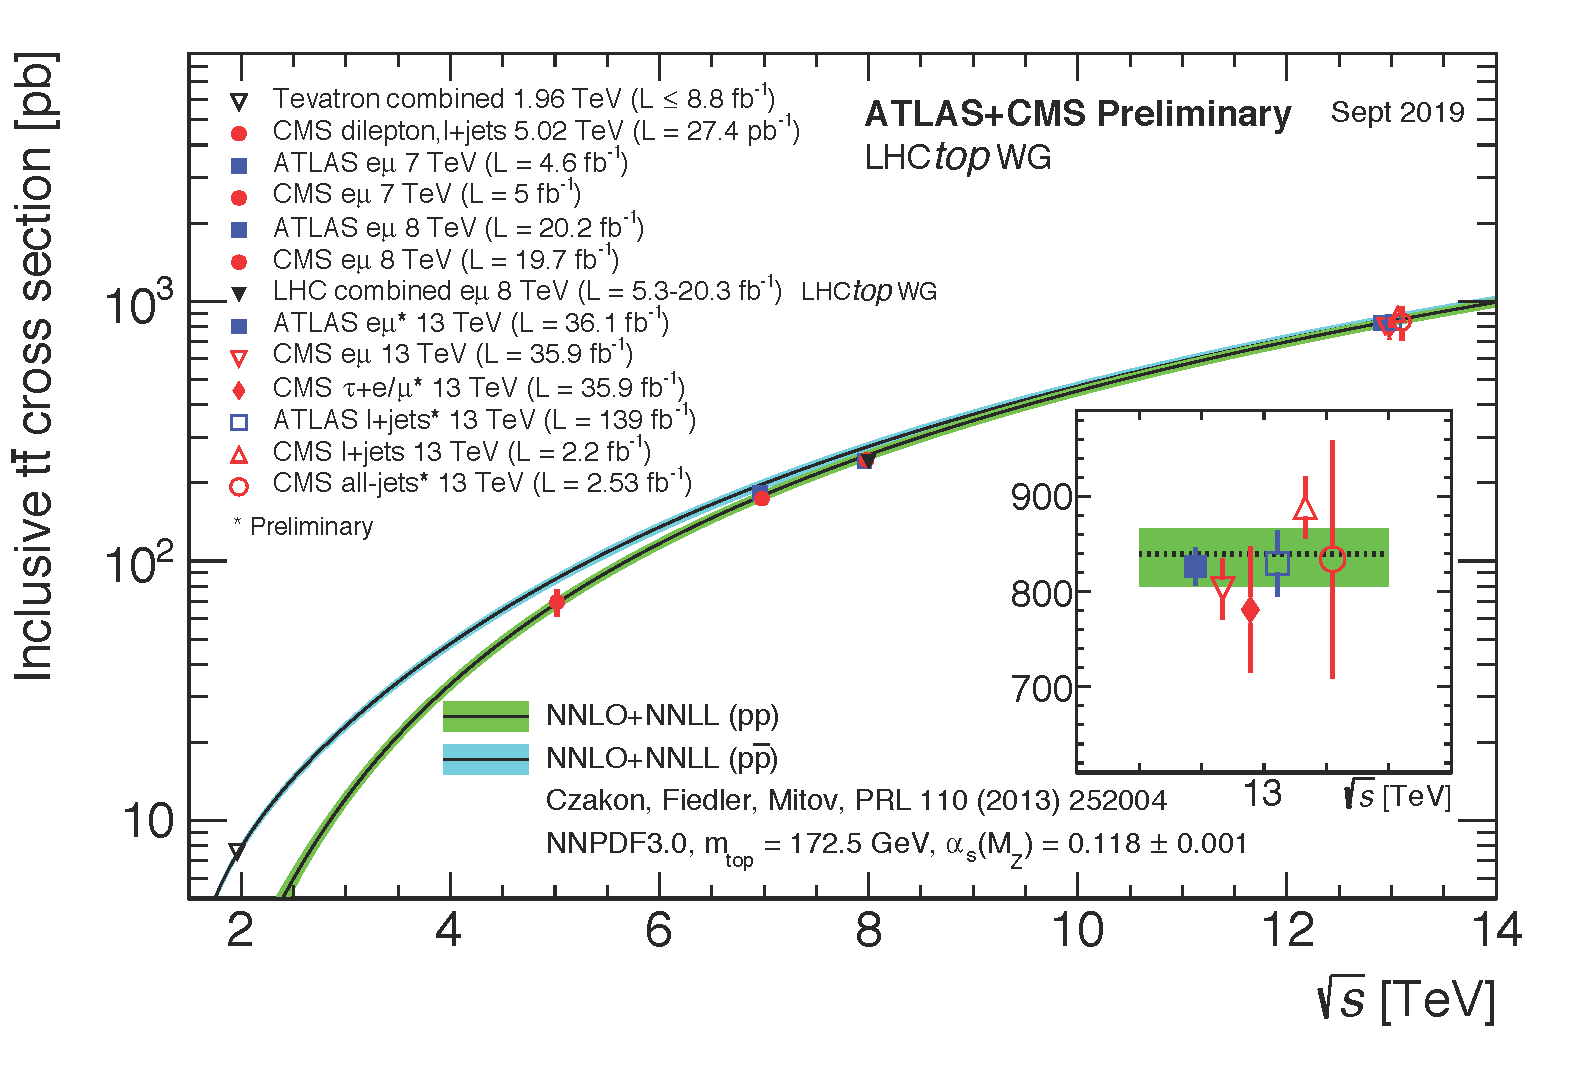
\includegraphics[height=0.7\textheight]{../../ThesisImages/ttprodxsec.png}
	\captionof{figure}{$t\bar{t}$ production cross section \href{https://twiki.cern.ch/twiki/bin/view/LHCPhysics/LHCTopWGSummaryPlots}{[TopWGSummaryPlots]}}
}

\frame{\frametitle{Top Quark Decays}
\begin{columns}
\begin{column}{0.5\textwidth}
\begin{itemize}
\item Standard model top branching ratio to bW $\simeq 100\%$
\end{itemize}
\centering
 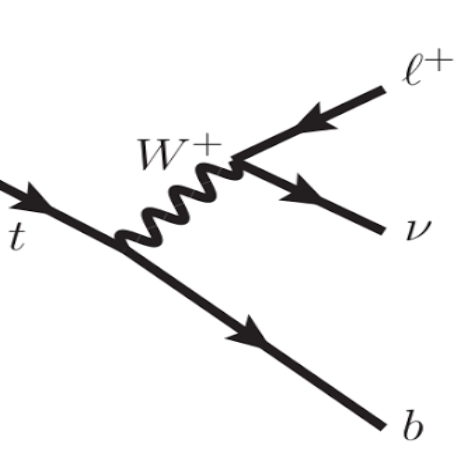
\includegraphics[width=0.7\textwidth]{../../ThesisImages/topdecay.png}
 \captionof{figure}{Leptonic final state diagram for a top decay}
\end{column}
\begin{column}{0.5\textwidth}  %%<--- here
     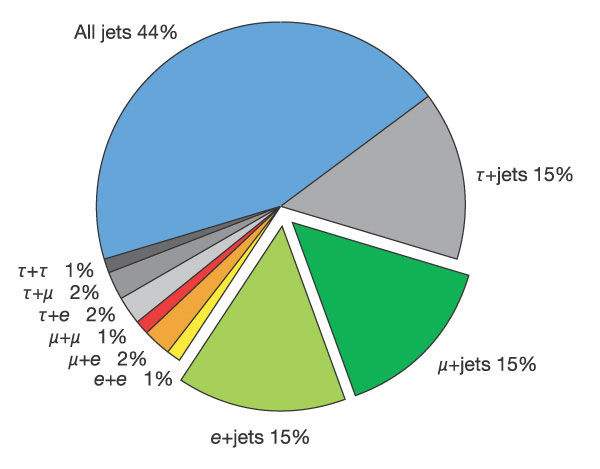
\includegraphics[width=1.1\textwidth]{../../ThesisImages/topdecayproducts.jpg}
    \captionof{figure}{Top quark pair decay final states \href{https://images.nature.com/full/nature-assets/nature/journal/v429/n6992/images/nature02589-f2.2.jpg}{[Nature]}}
\end{column}
\end{columns}
}

\frame{\frametitle{Top Quark Decays in the SM}
\centering
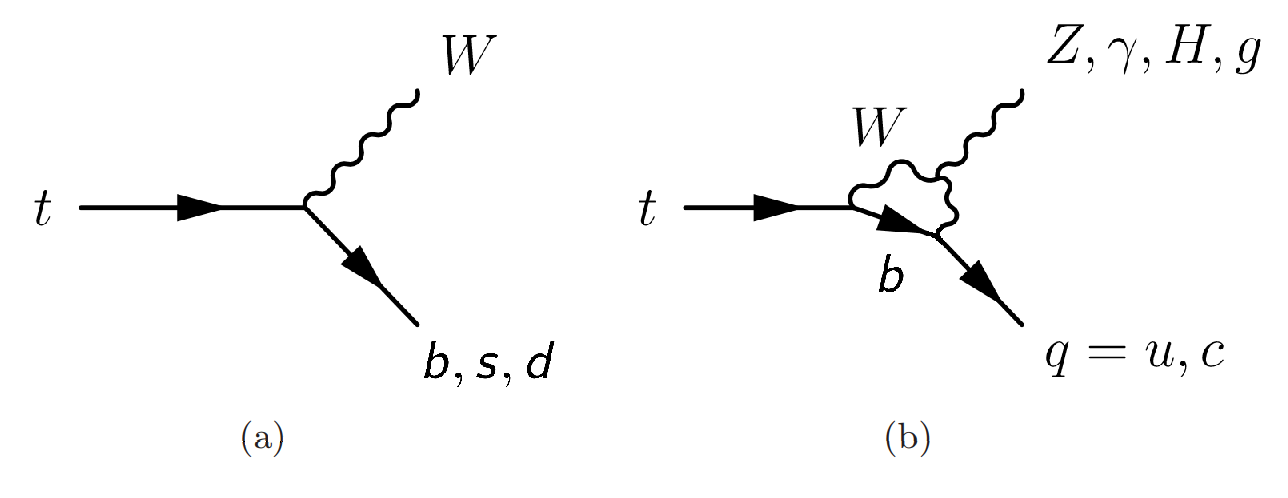
\includegraphics[width=1.\textwidth]{../../ThesisImages/SMTopDecays.png}

\begin{columns}
\begin{column}{0.5\textwidth}
\begin{itemize}
\item $t\rightarrow b W \approx 99.83\%$
\item $t\rightarrow s W \approx 0.16\%$
\item $t\rightarrow d W \approx 0.01\%$
\end{itemize}
\end{column}
\begin{column}{0.5\textwidth}
\begin{itemize}
\item $t\rightarrow q_{u,c} X\approx 10^{-17} - 10^{-12}$
\end{itemize}
\end{column}
\end{columns}

%\feynmandiagram [small,horizontal=a to b] {
%  a [particle=\(t\)] -- [fermion] b ,
% f1 [particle=\({b,s,d} \)] -- b -- [boson] f2 [ particle=\(W\)],
%};
}

%%%%%%%%%%%%%
\subsection{Historical Background}

\frame{\frametitle{GIM Mechanism}
\begin{itemize}
\item Cabibbo model - 3 quarks (u, d, s)
\item Studies of kaon decays showed the existence of $K^+ \rightarrow \mu^+ \nu_\mu$ but an absence of predicted $K_{L}^0 \rightarrow \mu^+ \mu^-$
\item Even in the absence of a tree level decay $K_{L}^0$ decay the box diagram would be possible through an exchange of W bosons
\item Weak neutral current interactions in the uds model  have the form
\[
u\bar{u}+ (d\bar{d}\cos^2\theta_C+s\bar{s}\sin^2\theta_C)) +(s\bar{d} + d\bar{s})sin\theta_C cos\theta_C
\]
\end{itemize}
\centering
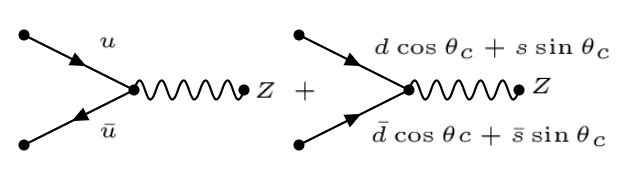
\includegraphics[width=0.45\textwidth]{../../ThesisImages/gimdeltaSa.png}
}

\frame{\frametitle{GIM Mechanism}
\centering
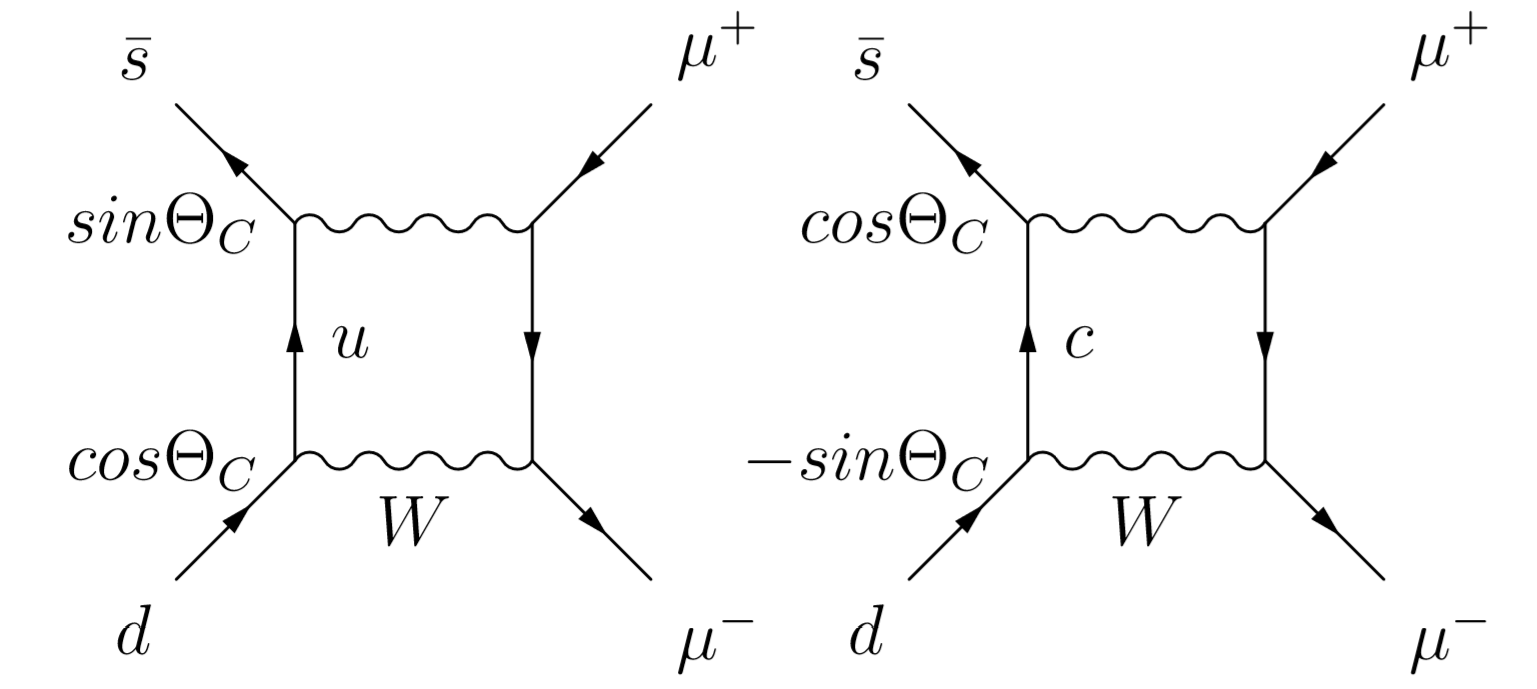
\includegraphics[width=.6\textwidth]{../../ThesisImages/GIMDiagrams.png}

\begin{itemize}
\item Glashow, Iliopoulos, and Maiani \href{https://journals.aps.org/prd/abstract/10.1103/PhysRevD.2.1285}{[Phys. Rev. D (1970)]} propose a machanism through which FCNCs are suppressed in loop diagrams
	\begin{itemize}
	\item Introduction of charm quark
	\end{itemize}
\item Kaon decays imply no neutral current/natural suppression of neutral current
\end{itemize}
}

\frame{\frametitle{GIM Mechanism}
\centering
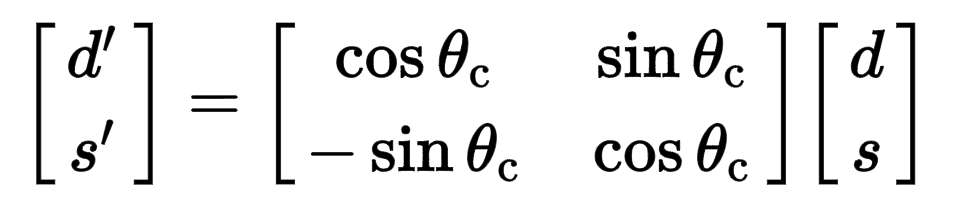
\includegraphics[width=.4\textwidth]{../../ThesisImages/cabibboangle.png}
\begin{itemize}
\item The addition of the charm changes our weak neutral current interactions
\item With four quarks the weak neutral interactions now have the form:
\[
u\bar{u} + c\bar{c} + (d\bar{d}+s\bar{s}) \cos^2\theta_C + (s\bar{s} + d\bar{d})\sin^2\theta_C +(s\bar{d} + d\bar{s} - d\bar{s} - s\bar{d})sin\theta_C cos\theta_C
\]
\item Flavor changing neutral current diagrams cancel out at tree level (as $m_{c} \rightarrow m_{u}$)
\end{itemize}
\centering
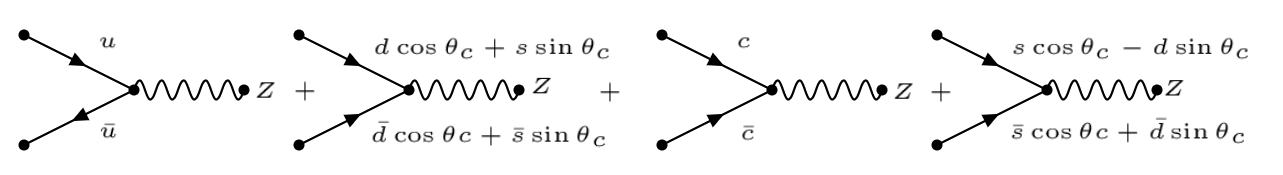
\includegraphics[width=0.9\textwidth]{../../ThesisImages/gimdeltaS.png}
}


\frame{\frametitle{CKM Matrix}
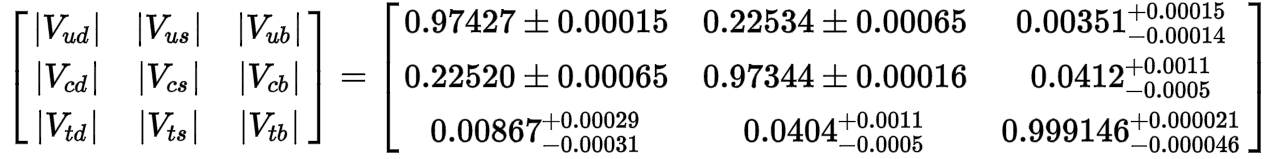
\includegraphics[width=1.\textwidth]{../../ThesisImages/CKMMatrix.png}
\captionof{figure}{CKM Matrix}
\begin{itemize}
\item Decay rates proportional to $|V_{tX}|^2$
\item Top decay through a $W^{\pm}$ boson is a charged current interaction. 
\item Flavor changing processes are proportional to off-diagonal elements of the CKM matrix
\item GIM/CKM suppression of these FCNC processes in the Standard Model make them unlikely to be seen without some new physics
\end{itemize}
}



%%%%%%%%%%%%%%%%%%%%%%%%%%%%%%%%%%%%%%%%%%%%%%%%%%%%%%%%%%%%%%%%%%%%

\section{Flavor Changing Neutral Current Searches with Top Quarks}

\subsection{Theory Predictions and Experimental Limits}


\frame{\frametitle{Top Flavor Changing Neutral Currents (FCNCs)}
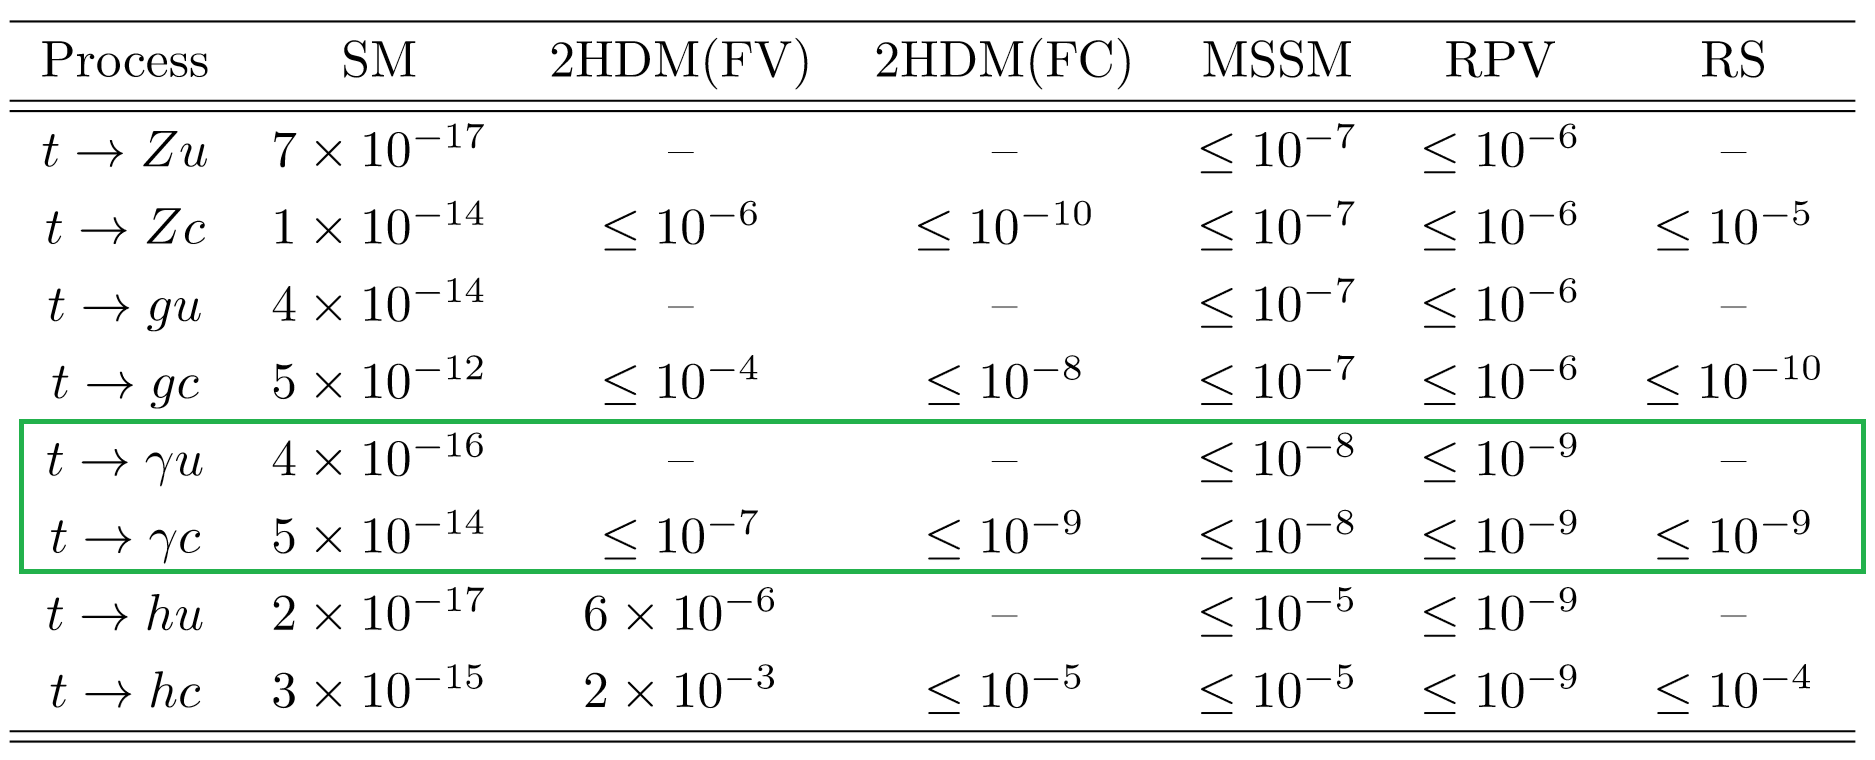
\includegraphics[width=1.\textwidth]{../../ThesisImages/ModelLimits.png}
\captionof{table}{Branching ratio enhancements in various beyond the standard model theories \href{https://arxiv.org/pdf/1311.2028.pdf}{[Snowmass Top Report]}}

}

\frame{\frametitle{Top Flavor Changing Neutral Currents}
\begin{itemize}
\item Current Limits on FCNC Decays
\end{itemize}
\centering
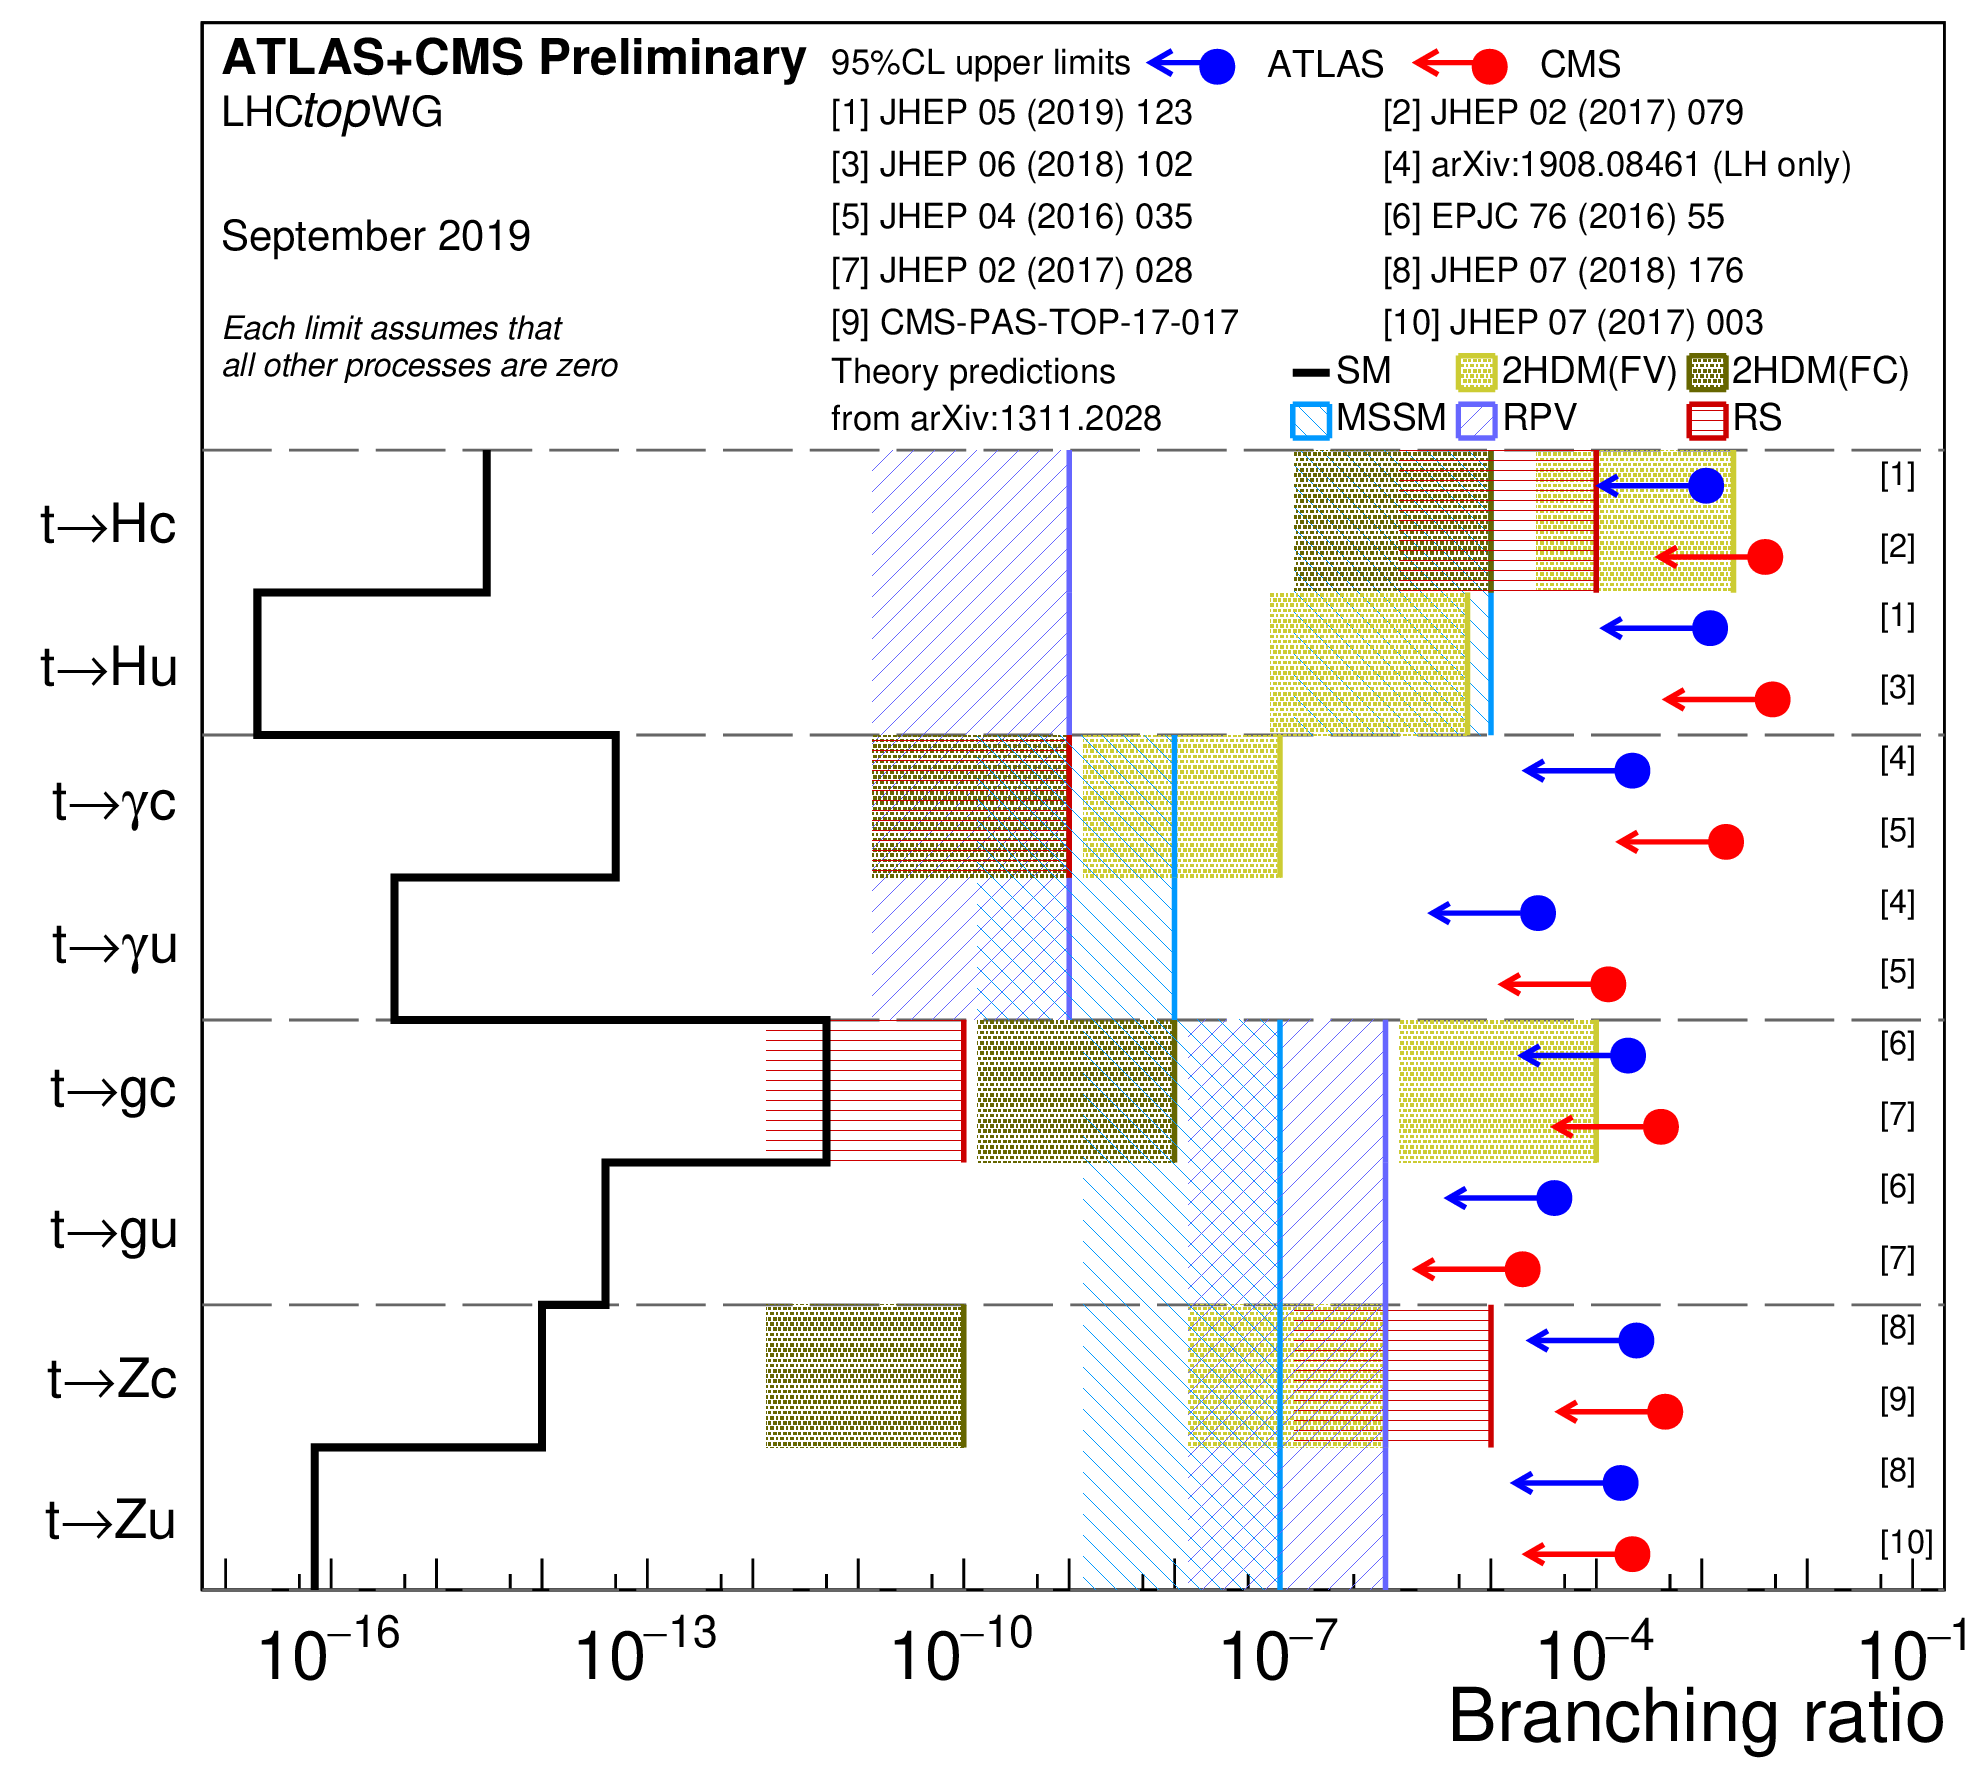
\includegraphics[width=0.55\textwidth]{../../ThesisImages/AllFCNCLimits.png}
\begin{itemize}
\item Limits on $t\rightarrow \gamma q$ processes: \href{https://arxiv.org/abs/1511.03951}{[JHEP 04 (2016) 035]}
	\begin{itemize}
	\item $t\rightarrow \gamma u < 1.3 x10^{-4}$
	\item $t\rightarrow \gamma c < 1.7 x 10^{-3}$
	\end{itemize}
\end{itemize}
}

\frame{\frametitle{Monte Carlo Production of FCNC Signal Samples}

\begin{itemize}
\item Due to the low cross sections we must create our own Monte Carlo Samples for our Signal
\item An effective field theory approach was taken in the creation of the model [Degrande et al. Phys. Rev. D 91, 034024 (2015)]
\item This model takes advantage of dimension-6 operators
\end{itemize}
\[ \mathcal{L}_{SM} = \mathcal{L}_{SM}^{(4)} + \mathcal{L}^{eff} \text{ where } \mathcal{L}^{eff} = \frac{1}{\Lambda^2} \sum_{k} C_{k}^{(6)}Q_{k}^{(6)}
\]
\[ \mathcal{L}^{eff}_{tq\gamma} =  C \sigma^{\mu\nu}q_{\nu}(\lambda^{L}_{ct}P_L + \lambda^{R}_{ct}P_{R}) t A_{\mu} +H.c.
\]
}

\frame{\frametitle{Top FCNC Signal Creation - Kinematic Checks}
%\centering
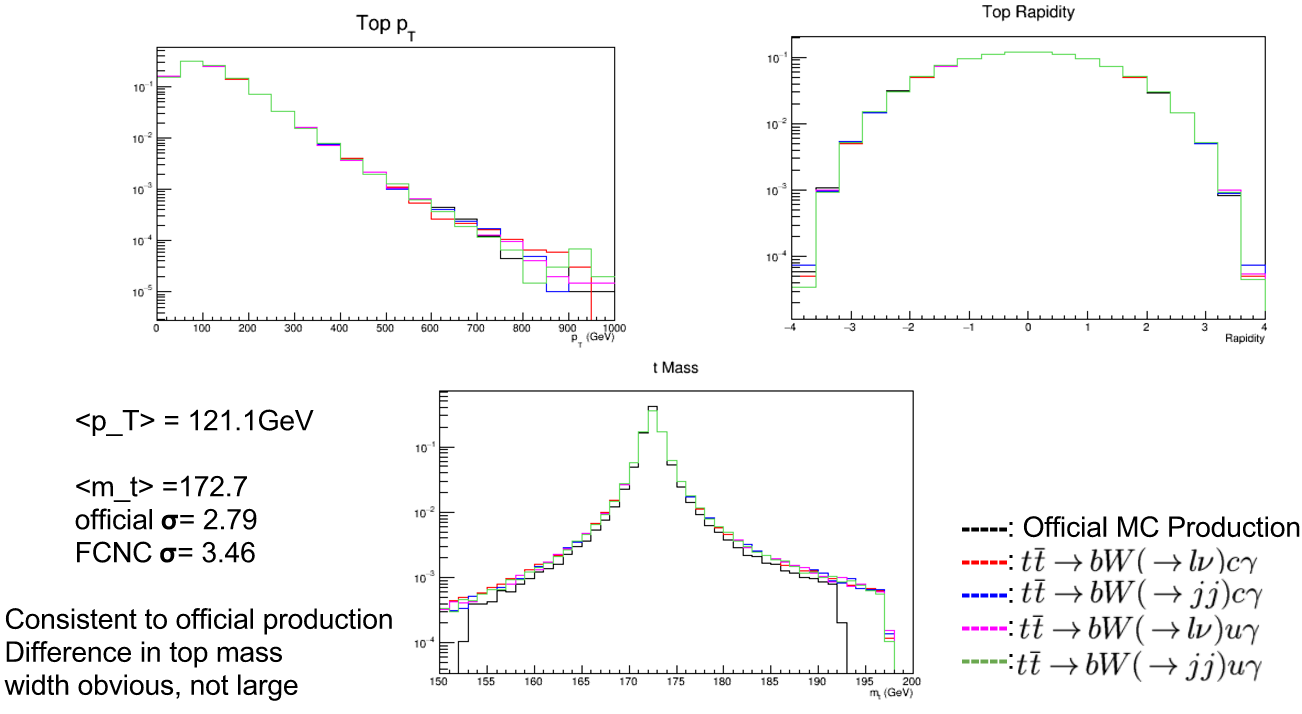
\includegraphics[width=1.\textwidth]{../../ThesisImages/FCNCValidation.png}
}

\frame{\frametitle{Top FCNC Signal Creation - Kinematic Checks}
%\centering
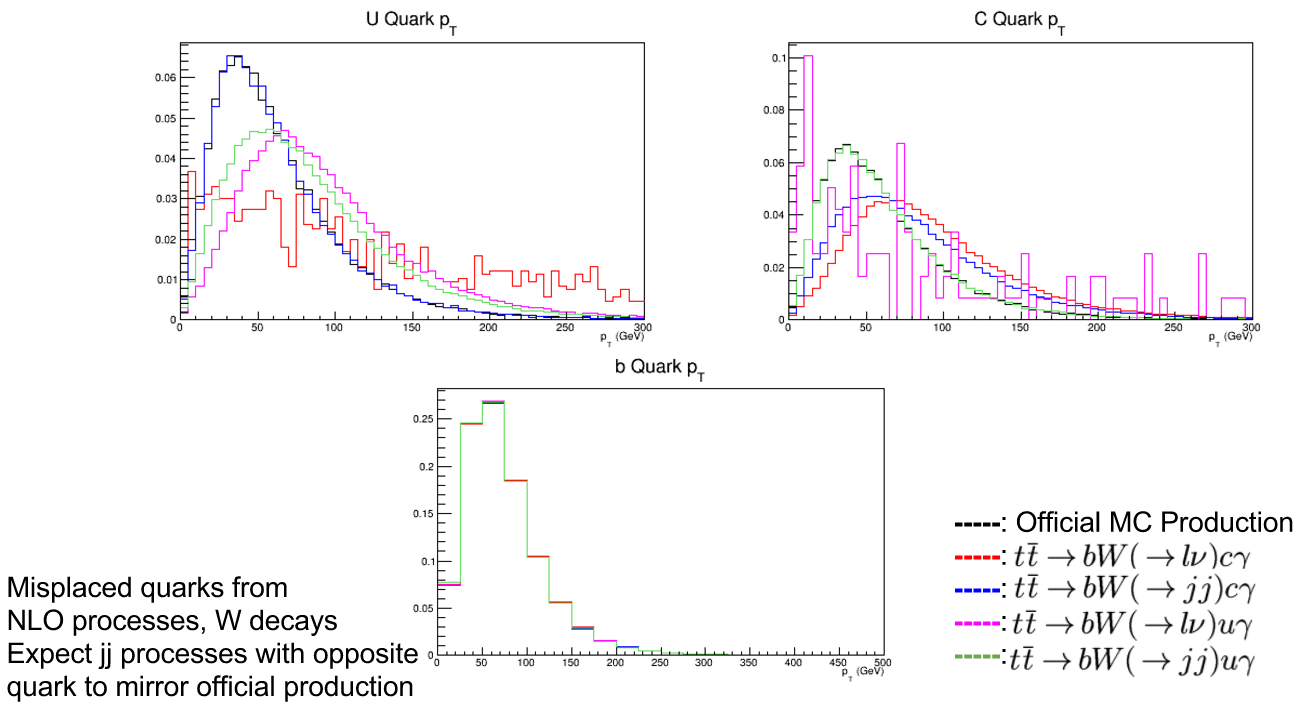
\includegraphics[width=1.\textwidth]{../../ThesisImages/FCNCValidation2.png}
}


\subsection{FCNC at the LHC}
\frame{\frametitle{FCNC: What are we looking for? $t\bar{t}\rightarrow W (\rightarrow l \nu) b+ q\gamma$}
\begin{itemize}
\item Final state topology
	\begin{itemize}
	\item One Neutrino, from W
	\item One Lepton, from W
	\item One B-jet, SM top
	\item One Photon, FCNC Top
	\item One Jet, FCNC Top
	\end{itemize}
\end{itemize}
\centering
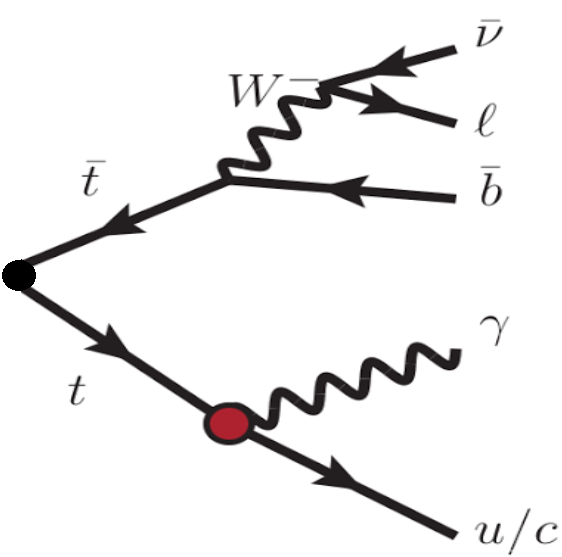
\includegraphics[width=0.4\textwidth]{../../ThesisImages/fcncttbar.png}
}
%%%%%%%%%%%%%%%%%%%%%%%%%%%%%%%%%%%%%%%%%%%%%%%%%%%%%

\section{The Large Hadron Collider and the ATLAS Detector}
\subsection{The LHC}
\frame{\frametitle{The Large Hadron Collider (LHC)}
\begin{itemize}
\item $27km$ ring beneath France-Switzerland border
\item 4 Major Experiments
\item Collides protons at $\sqrt{s}=13 TeV $ 
\end{itemize}
\centering
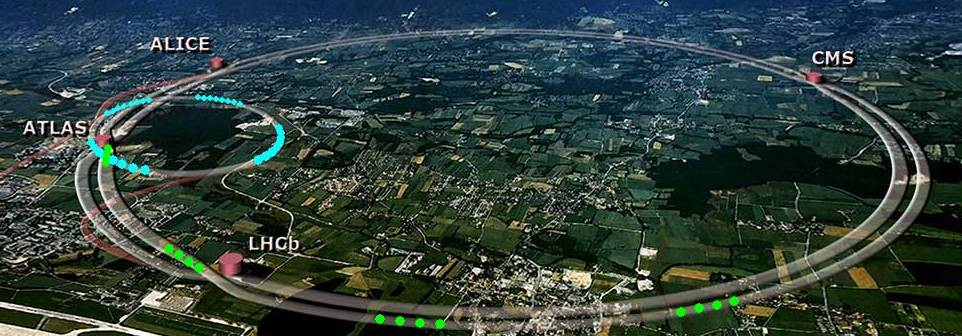
\includegraphics[width=0.9\textwidth]{../../ThesisImages/lhc-aerial.jpg}
}



\subsection{ATLAS}
\frame{\frametitle{The ATLAS Detector}
\centering 
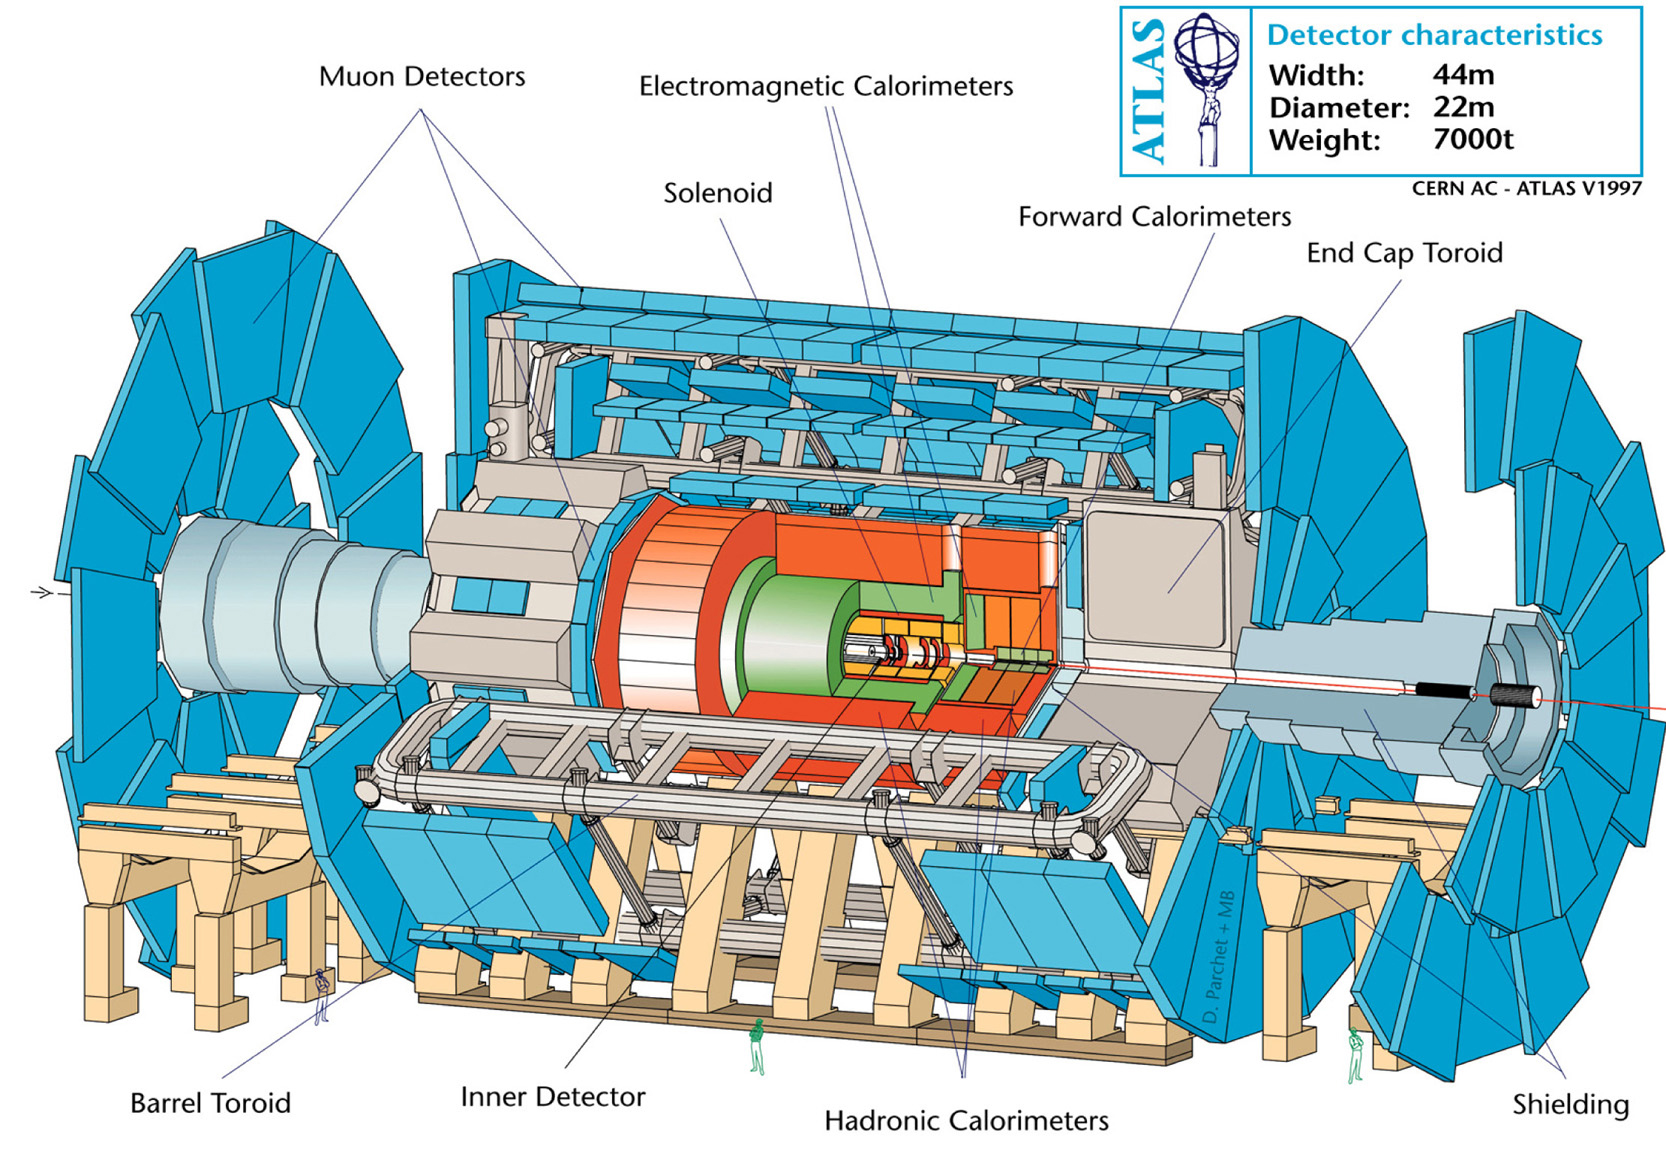
\includegraphics[width=1.\textwidth]{../../ThesisImages/atlasdet.jpg}
}

\frame{\frametitle{Particles in ATLAS}
\centering 
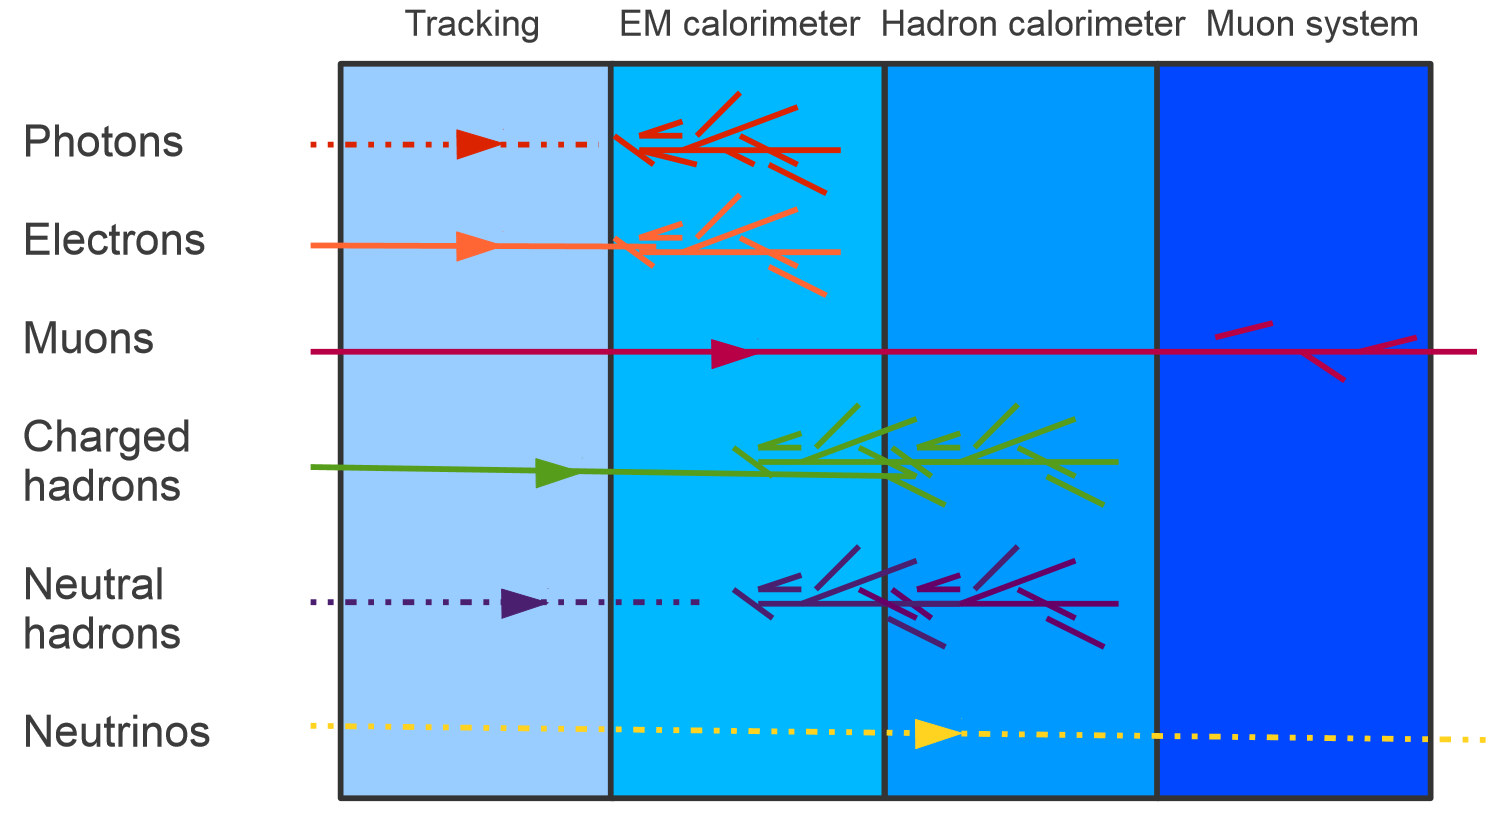
\includegraphics[width=1.\textwidth]{../../ThesisImages/ParticlesInDetector.png}
\newline
*Courtesy of Liza Brost
}

\frame{\frametitle{Jets}
\begin{itemize}
\item Quarks leaving from the interaction form into narrow cones of particles
\item Jets are identified with the anti-$\text{k}_T$ algorithm
\end{itemize}
\centering
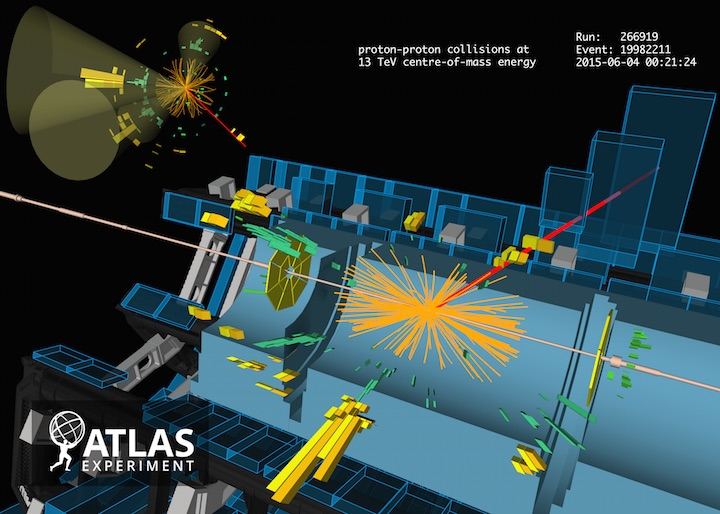
\includegraphics[width=.45\textwidth]{../../ThesisImages/ttbarevent.png}
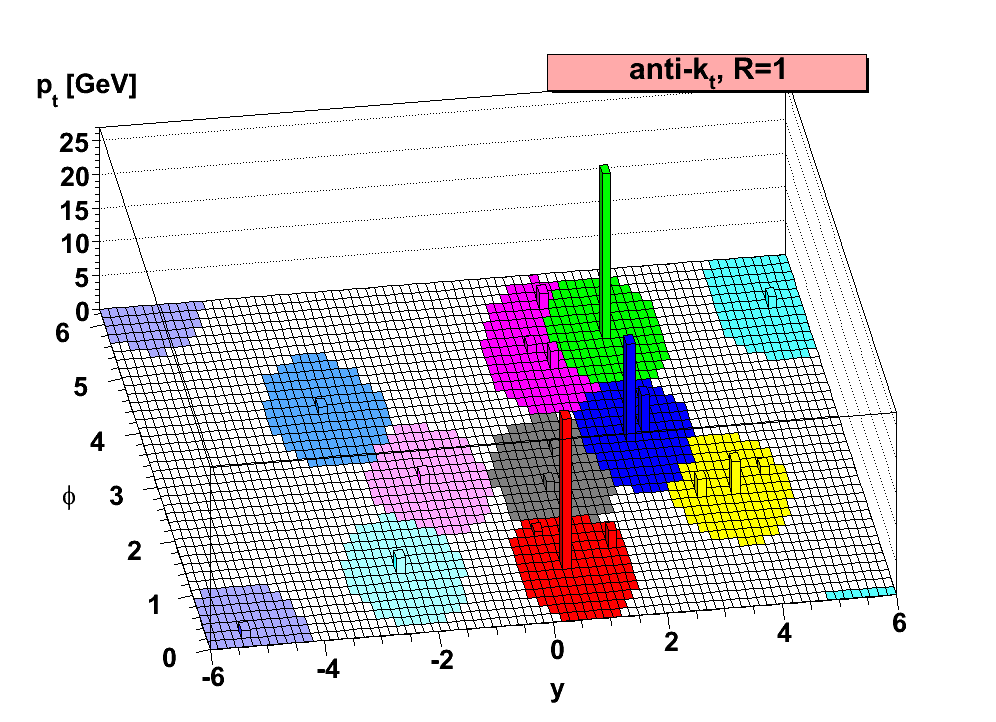
\includegraphics[width=.45\textwidth]{../../ThesisImages/AntiKtJets.png}
}

\subsection{ATLAS Data}

\frame{\frametitle{ATLAS Data}
\centering
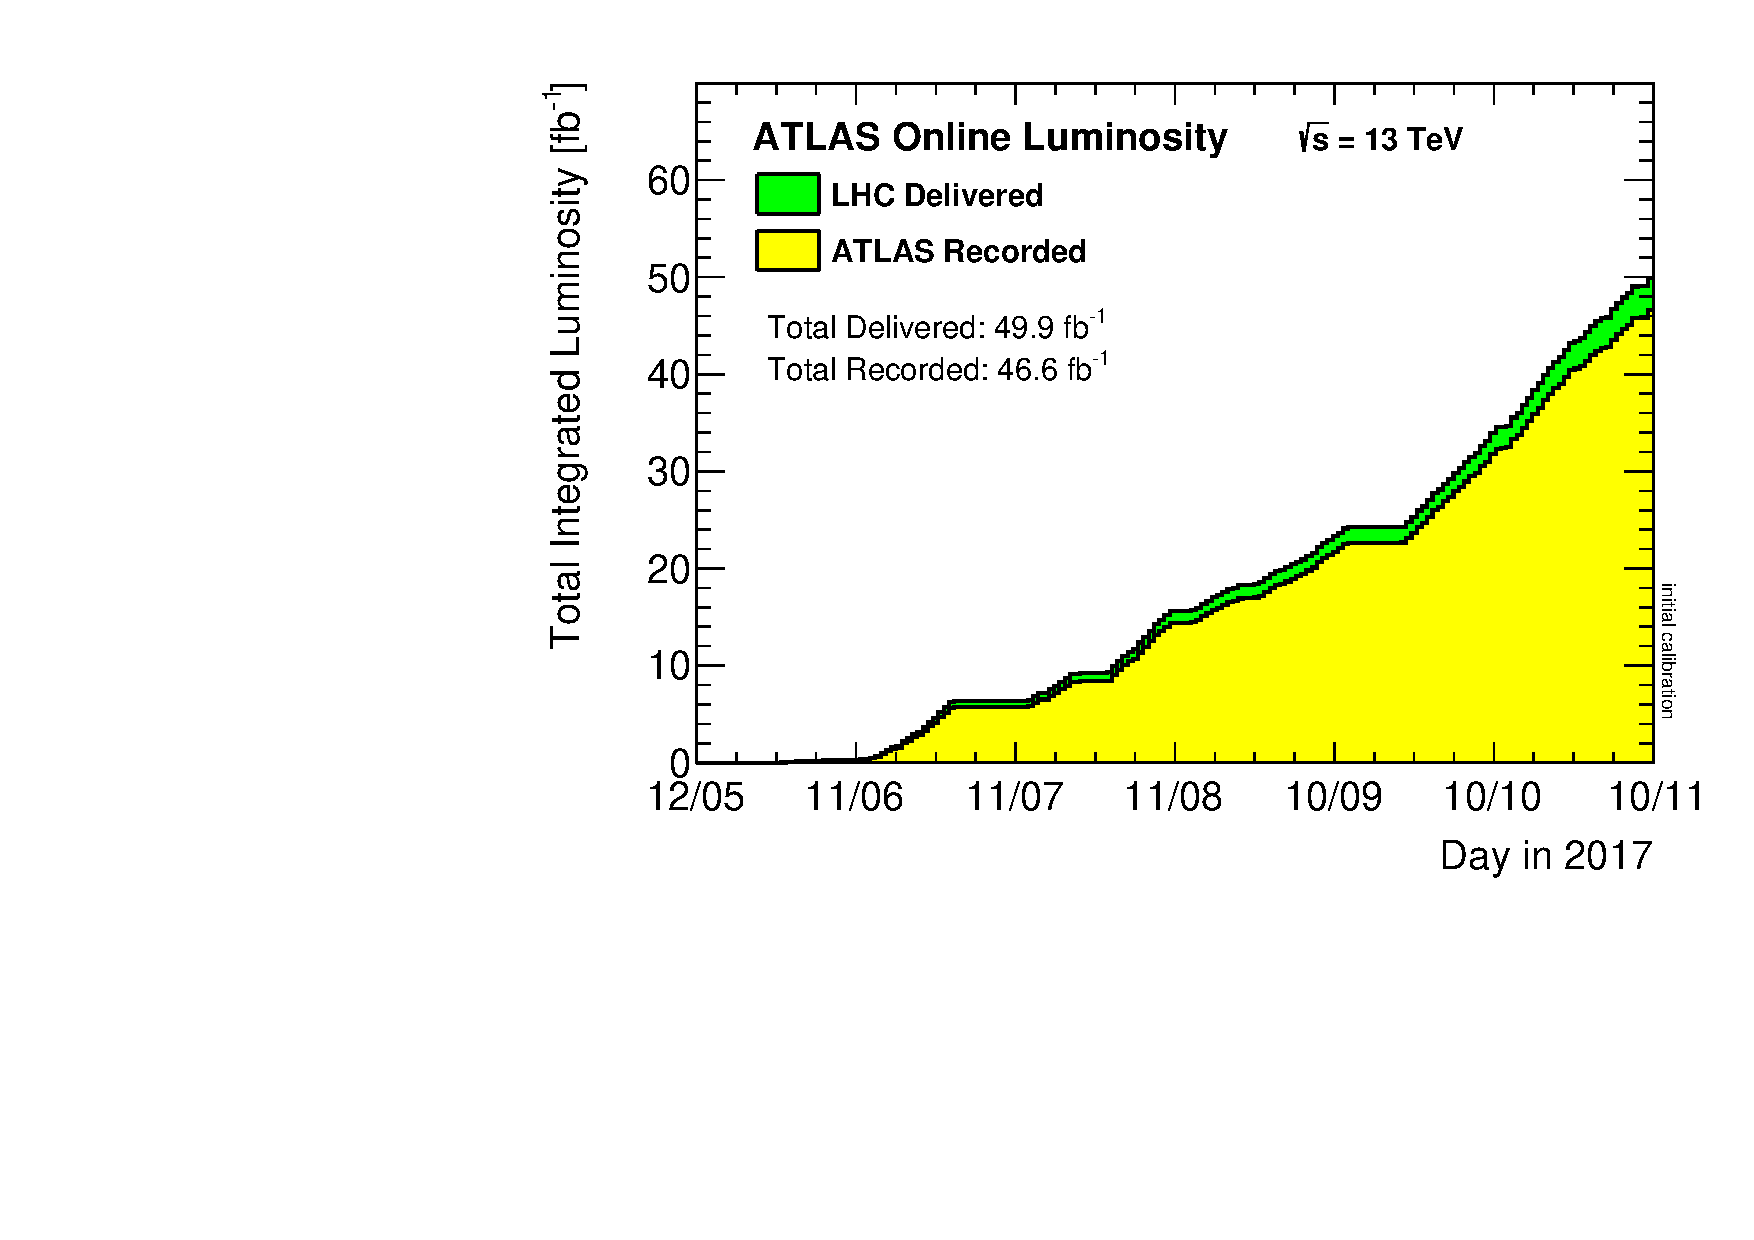
\includegraphics[width=0.8\textwidth]{../../ThesisImages/2017LumiByDay.pdf}
\begin{itemize}
\item Total recorded integrated luminosity at $\sqrt{s} = 13TeV$:  $86.4\text{fb}^{-1}$
\end{itemize}
}

\frame{\frametitle{What's in the data?}
\begin{columns}
\begin{column}{0.5\textwidth}
\centering 
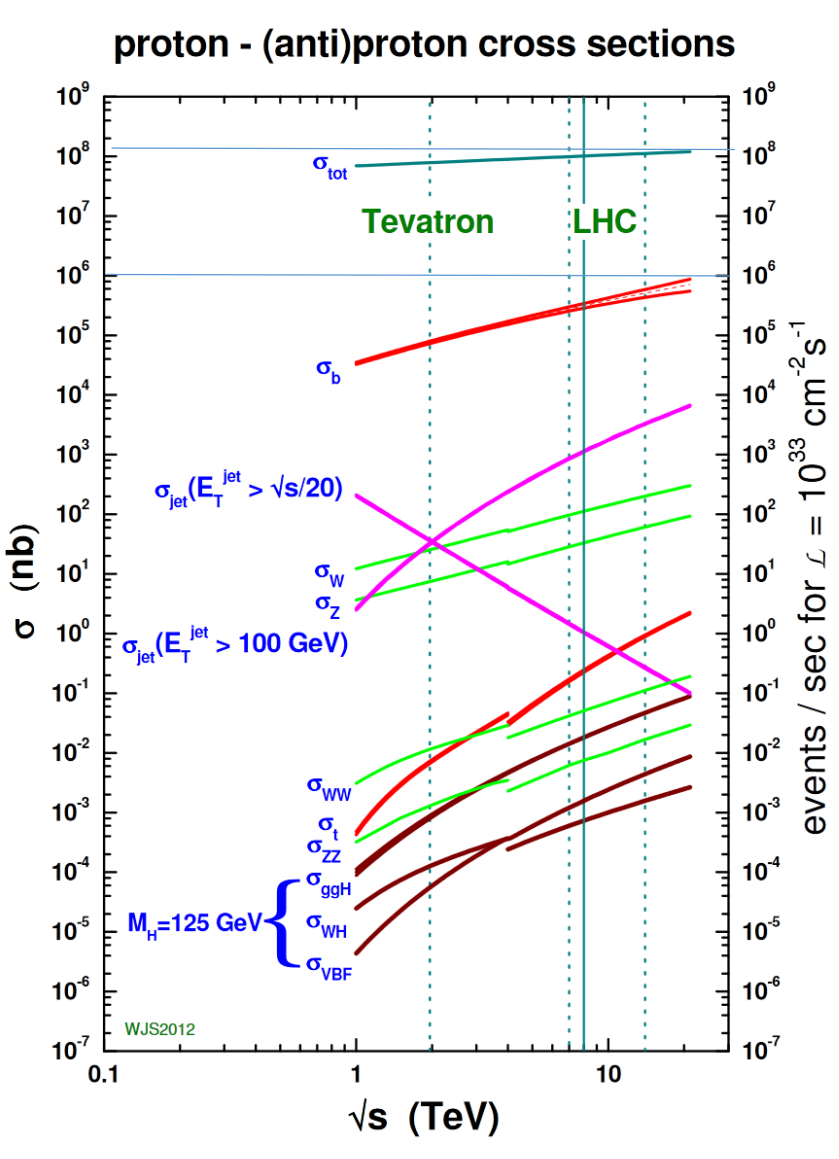
\includegraphics[width=1.\textwidth]{../../ThesisImages/HardScatCrosSecs.png}
\end{column}
\begin{column}{0.5\textwidth}
\begin{itemize}
\item The number of events we see is $N=\sigma L$
\item $\sigma_{t\bar{t}}=$ 831.76pb
\item $N_{t\bar{t}} \approx 72x10^6$
\item $N_{tot} \approx 8.6x10^{15}$ events produced during the 13TeV data runs
\end{itemize}
\end{column}
\end{columns}
}


\subsection{Trigger and Data Acquisition}

\frame{\frametitle{Data Acquisition}
\begin{itemize}
\item The LHC provides around 600 million interactions every second
\item Raw event data is about $1MB \Rightarrow 600TB$ event data per second
\item Absolutely impossible to save this amount of data
\item We need a way to pick out interesting events to save
\end{itemize}
}

\frame{\frametitle{Trigger System}
\centering 
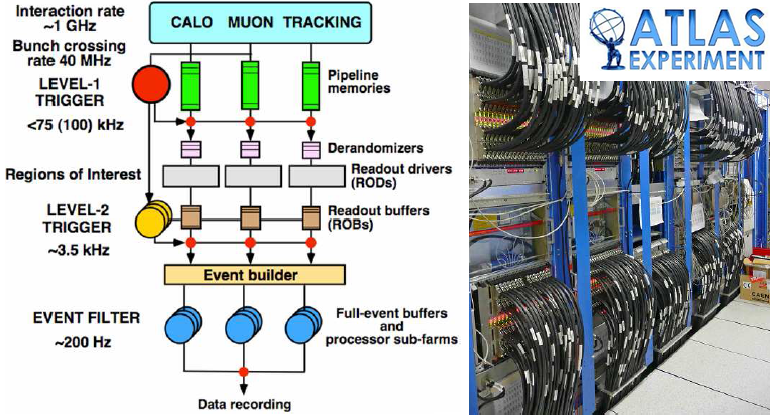
\includegraphics[width=0.6\textwidth]{../../ThesisImages/AtlasTrigger.png}
\begin{itemize}
\item We look for events with compelling topologies
	\begin{itemize}
	\item Leptons, High Energy Events, Missing Energy, etc.
	\end{itemize}
\item We only write these interesting events reducing $GHz$ interaction rate to around $200Hz$ to disk
\end{itemize}
}

%%%Now that we know what we're seeing lets look at what we're looking for

%%%%%%%%%%%%%%%%%%%%%%%%%%%%%%%%%%%%%%%%%%%%%%%%%%%%%%%%%%%%%%%%%
\section{Searching for Flavor Changing Neutral Current Signatures}

\subsection{FCNCs with Photons}

\subsection{Object Preselection Cuts}


\frame{\frametitle{Object Preselection}
\begin{itemize}
\item We preselect events with objects that look like our expected topology
\item Require:
	\begin{itemize}
	\item Exactly one lepton (e or $\mu$) $\geq$ 25 GeV
	\item Exactly one Good photon $\geq$ 25GeV
	\item Missing Transverse Energy $\geq$ 30GeV
	\item $\geq 2$ Jets (at least one being b-tagged)
	\end{itemize}
\item All following plots will have signal scaled to $1\%$ of $\sigma_{t\bar{t}}$, MC scaled to $36.07fb^{-1}$
\end{itemize}
}

\frame{\frametitle{Background Processes}
\begin{itemize}
\item Due to all of the processes at hadron colliders it is important to model similar event topologies well.
\item Major backgrounds include $t\bar{t}$, W+Jets, Z+Jets, + processes with an associated photon
\end{itemize}
\centering
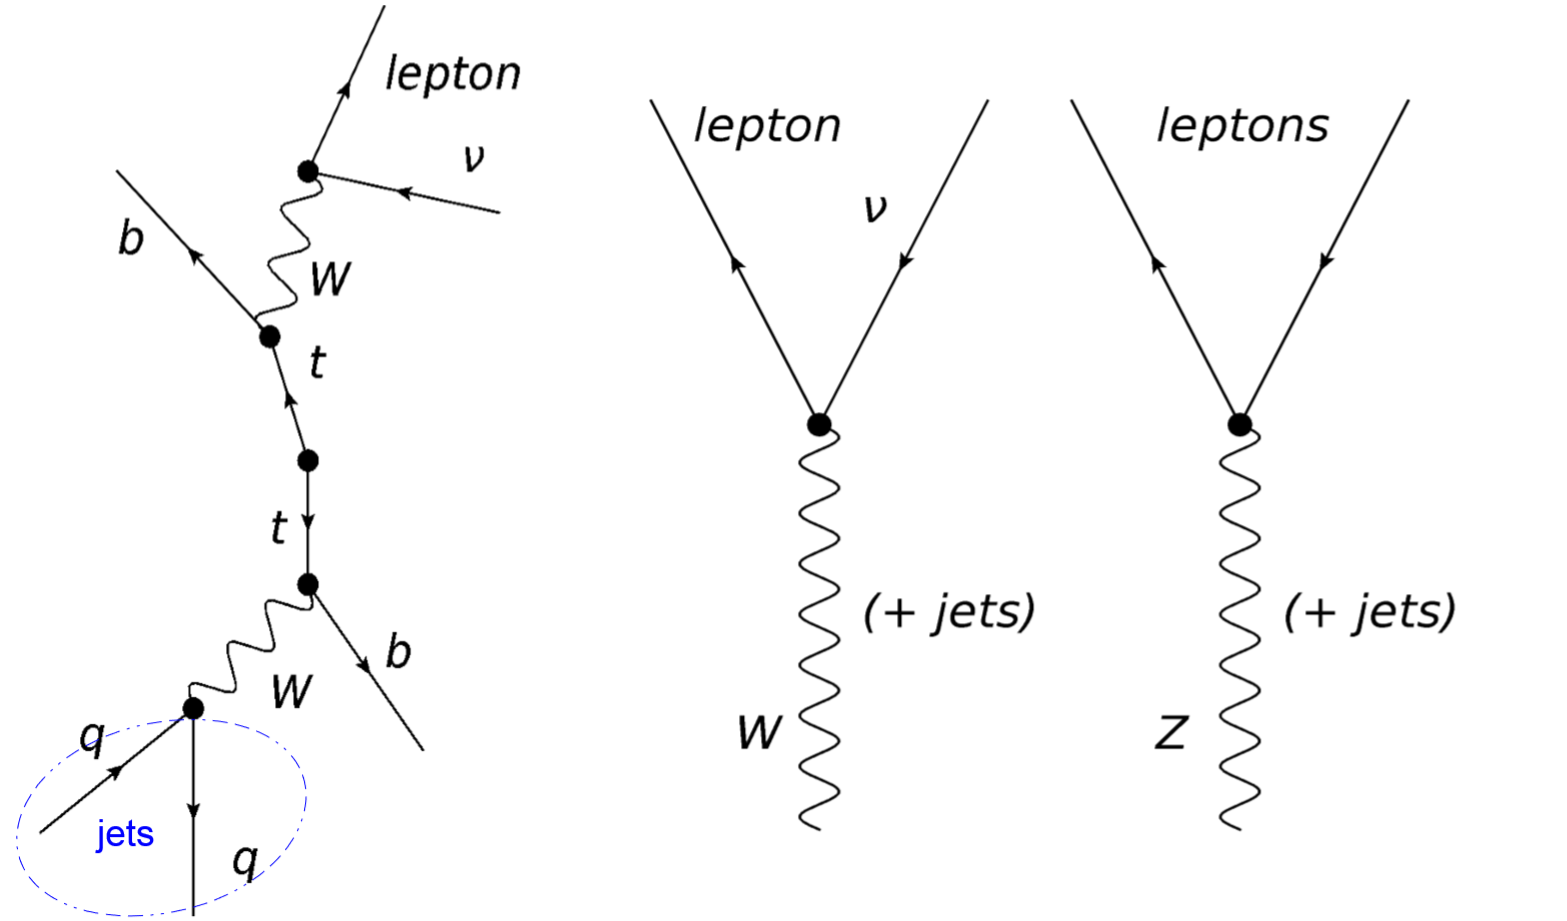
\includegraphics[width=0.7\textwidth]{../../ThesisImages/backgrounds.png}
}

\frame{\frametitle{Preselection Objects}

\begin{columns}
\begin{column}{0.02\textwidth}

\rotatebox{90}{Muon Channel \qquad  Electron Channel} 
%\rotatebox{90}{Muon Channel        } 
\end{column}
\begin{column}{0.33\textwidth}
\begin{itemize}
\item  Leading Jet $p_T$
\end{itemize}
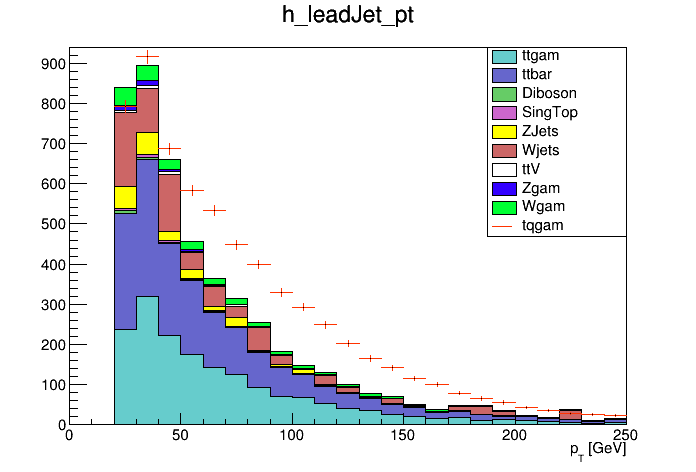
\includegraphics[width=1.1\textwidth]{../../ThesisImages/plotsloose/el_h_leadJet_pt.png} \\
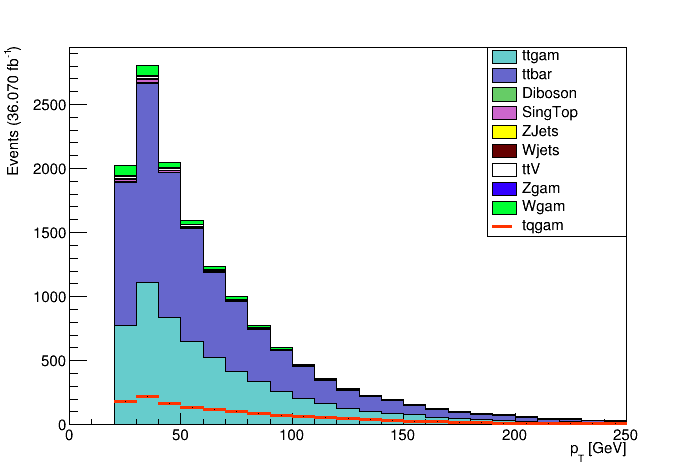
\includegraphics[width=1.1\textwidth]{../../ThesisImages/plotsloose/mu_h_leadJet_pt.png}
\end{column}
\begin{column}{0.33\textwidth}
\begin{itemize}
\item Photons
\end{itemize}
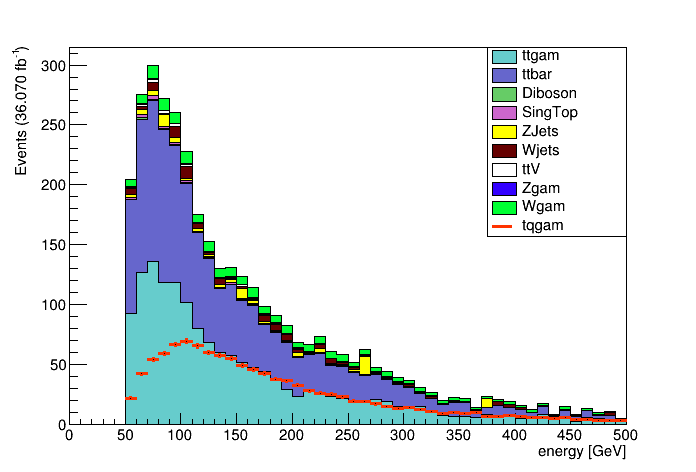
\includegraphics[width=1.1\textwidth]{../../ThesisImages/plotsloose/el_h_photon_e.png} \\
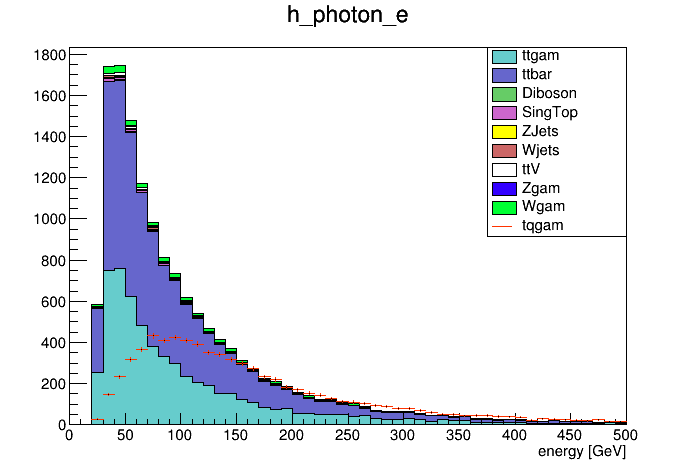
\includegraphics[width=1.1\textwidth]{../../ThesisImages/plotsloose/mu_h_photon_e.png}
\end{column}
\begin{column}{0.33\textwidth}
\begin{itemize}
\item Leptons
\end{itemize}
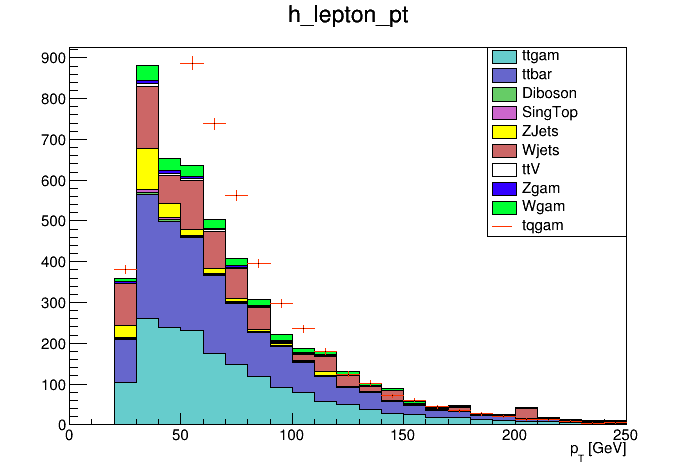
\includegraphics[width=1.1\textwidth]{../../ThesisImages/plotsloose/el_h_lepton_pt.png}\\
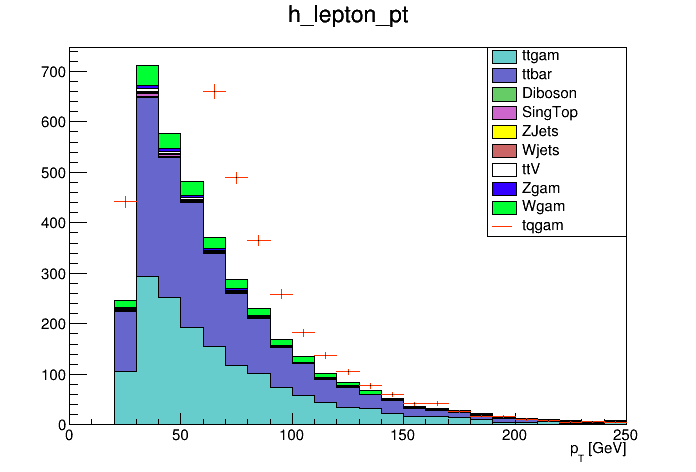
\includegraphics[width=1.1\textwidth]{../../ThesisImages/plotsloose/mu_h_lepton_pt.png}
\end{column}
\end{columns}

}

\subsection{Top and Neutrino Reconstruction}
\frame{\frametitle{Where are the Tops?}
\begin{itemize}
\item Must be 'reconstructed' from these objects as well as b-jets and $E_T^{miss}$
\item $E_T^{miss}$ is calculated to balance the event energy in the transverse plane of the detector
\item The other particles are combined in the only way the signal topology would allow two top quark candidates
\begin{itemize}
\item Standard model top candidate: b-jet + lepton + neutrino 
\item FCNC Top: Photon + Light Jet
\end{itemize}
\end{itemize}
}

\frame{\frametitle{Neutrinos}
\begin{itemize}
\item All missing energy in signal topology is from neutrino
\item We have $E_T^{miss}$ and its' direction   
\begin{itemize}
\item Can calulate  $E_{Tx}^{miss}$ and  $E_{Ty}^{miss}$ easily
\item Ambiguous direction along the z-axis
\end{itemize}
\item A minimization of this $\chi^2$ will allow us to determine the z momentum of the neutrino: $\chi^2 = \frac{(m_{b,l,\nu}-m_t)^2}{\sigma^2_{SMtop}}+\frac{(m_{l,\nu}-m_W)^2}{\sigma^2_W} $
\end{itemize}

%\[ \chi^2 = \frac{(m_{b,l,\nu}-m_t)^2}{\sigma^2_{SMtop}}+\frac{(m_{l,\nu}-m_W)^2}{\sigma^2_W}  \]
\begin{columns}
\begin{column}{0.5\textwidth}
\centering
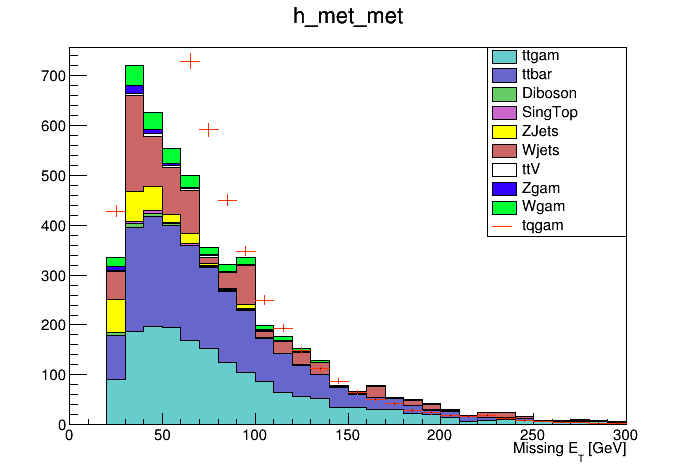
\includegraphics[width=.9\textwidth]{../../ThesisImages/plotsloose/el_h_met_met.png}
\captionof{figure}{e-channel $E_T^{miss}$ distribution}
\end{column} 
\begin{column}{0.5\textwidth}
\centering
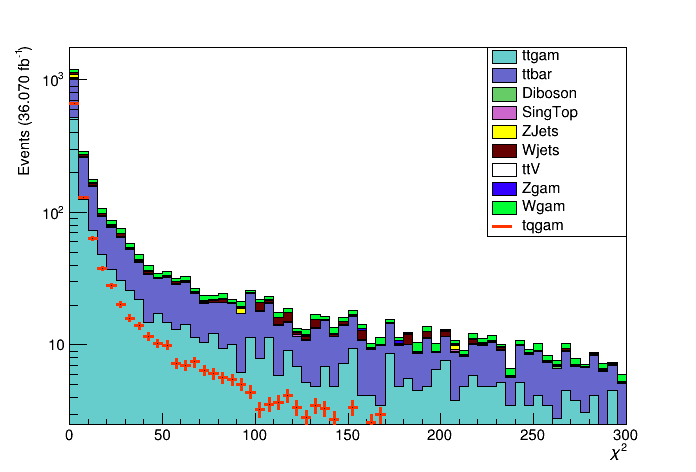
\includegraphics[width=.9\textwidth]{../../ThesisImages/plotsloose/el_h_min_chi2.png}
\captionof{figure}{e-channel $\chi^2$ distribution}
\end{column}
\end{columns}
}

\frame{\frametitle{Reconstructed Tops}
\begin{columns}
\begin{column}{0.02\textwidth}
\rotatebox{90}{Muon Channel \qquad  Electron Channel} 
\end{column}
\begin{column}{0.5\textwidth}
\begin{itemize}
\item SM Top
\end{itemize}
\centering
\includegraphics[width=.9\textwidth]{../../ThesisImages/plotsloose/el_h_sm_top_m.png}\\
\includegraphics[width=.9\textwidth]{../../ThesisImages/plotsloose/mu_h_sm_top_m.png}
\end{column} 
\begin{column}{0.5\textwidth}
\begin{itemize}
\item FCNC Top
\end{itemize}
\centering
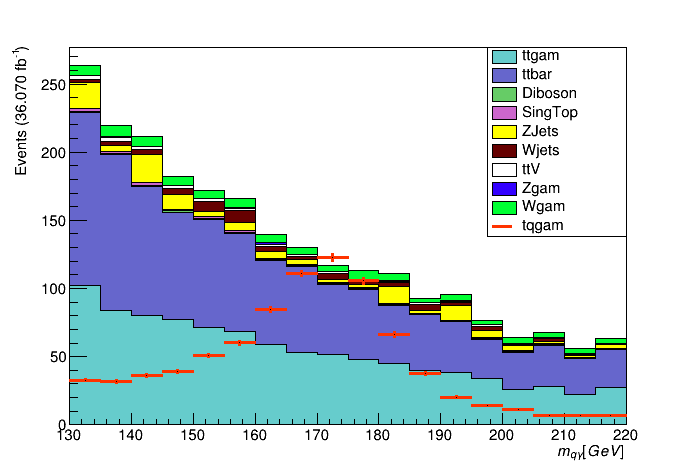
\includegraphics[width=.9\textwidth]{../../ThesisImages/plotsloose/el_h_qgam_m.png}\\
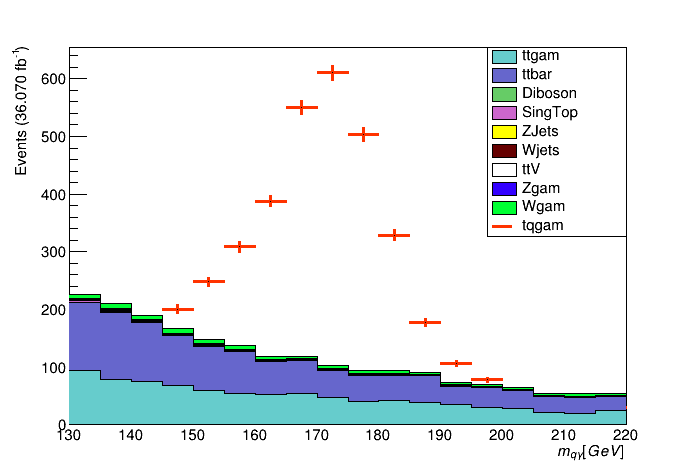
\includegraphics[width=.9\textwidth]{../../ThesisImages/plotsloose/mu_h_qgam_m.png}
\end{column}
\end{columns}
}


\frame{\frametitle{Thinning Out Backgrounds}
\begin{columns}
\begin{column}{0.02\textwidth}
\rotatebox{90}{Muon Channel \qquad  Electron Channel} 
\end{column}
\begin{column}{0.5\textwidth}
\begin{itemize}
\item Reconstructing Z mass
\end{itemize}
\centering
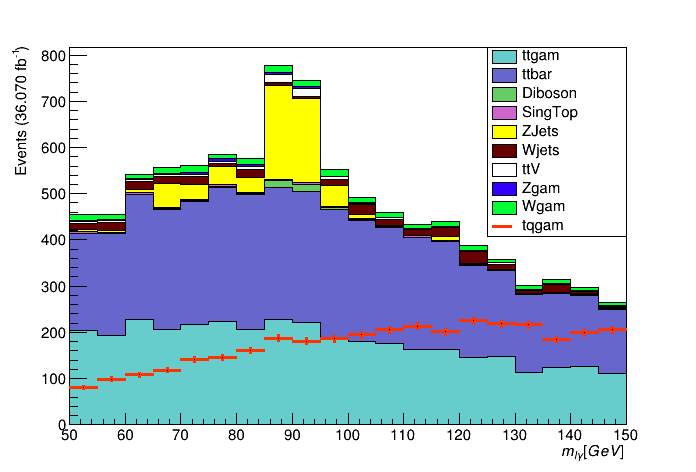
\includegraphics[width=.9\textwidth]{../../ThesisImages/plotsloose/el_h_lgam_m.png}\\
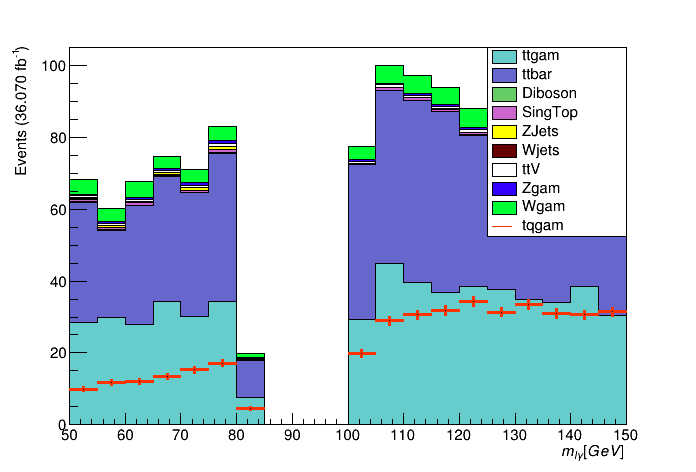
\includegraphics[width=.9\textwidth]{../../ThesisImages/plotsloose/mu_h_lgam_m.png}
\end{column} 
\begin{column}{0.5\textwidth}
\begin{itemize}
\item Number of BJets
\end{itemize}
\centering
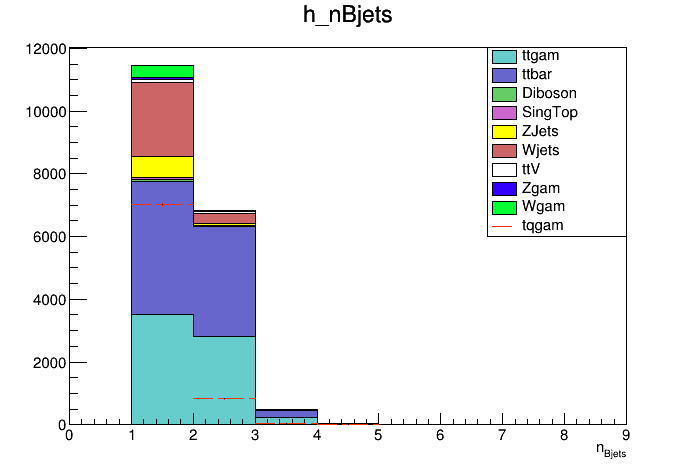
\includegraphics[width=.9\textwidth]{../../ThesisImages/plotsloose/el_h_nBjets.png}\\
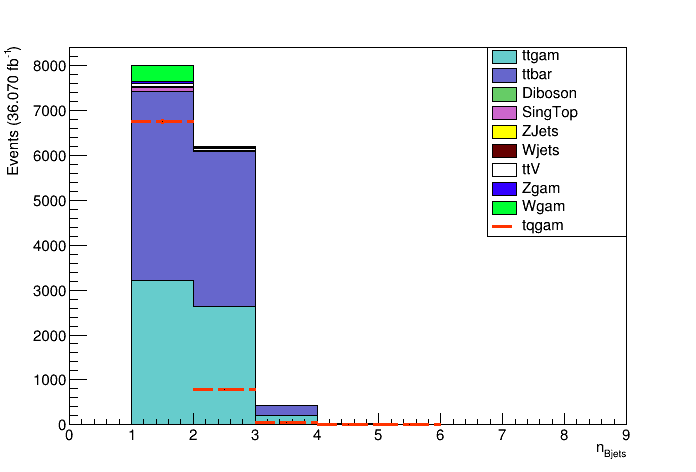
\includegraphics[width=.9\textwidth]{../../ThesisImages/plotsloose/mu_h_nBjets.png}
\end{column}
\end{columns}
}

\frame{\frametitle{Thinning Out Backgrounds: SM Top ($m_{l \nu b}$)}
\begin{columns}
\begin{column}{0.02\textwidth}
\rotatebox{90}{Muon Channel \qquad  Electron Channel} 
\end{column}
\begin{column}{0.5\textwidth}
\begin{itemize}
\item Before Z-mass, Bjet cuts
\end{itemize}
\centering
\includegraphics[width=.9\textwidth]{../../ThesisImages/plotsloose/el_h_sm_top_m.png}\\
\includegraphics[width=.9\textwidth]{../../ThesisImages/plotsloose/mu_h_sm_top_m.png}
\end{column} 
\begin{column}{0.5\textwidth}
\begin{itemize}
\item After Cuts
\end{itemize}
\centering
\includegraphics[width=.9\textwidth]{../../ThesisImages/plotsstrict/el_h_sm_top_m.png}\\
\includegraphics[width=.9\textwidth]{../../ThesisImages/plotsstrict/mu_h_sm_top_m.png}
\end{column}
\end{columns}
}

\frame{\frametitle{Thinning Out Backgrounds: FCNC Top}
\begin{columns}
\begin{column}{0.02\textwidth}
\rotatebox{90}{Muon Channel \qquad  Electron Channel} 
\end{column}
\begin{column}{0.5\textwidth}
\begin{itemize}
\item Before Z-mass, Bjet cuts
\end{itemize}
\centering
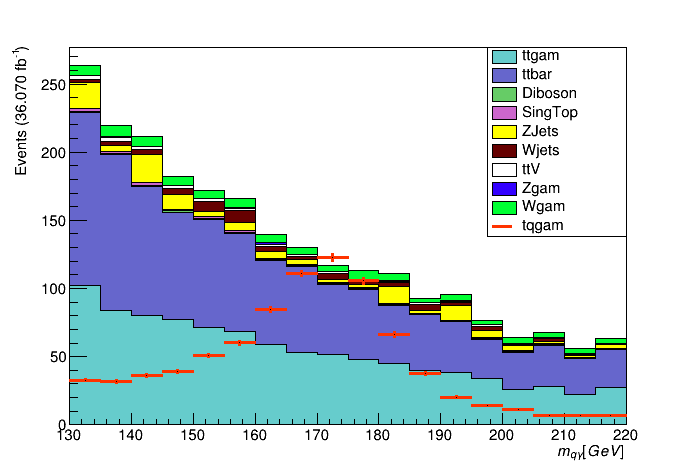
\includegraphics[width=.9\textwidth]{../../ThesisImages/plotsloose/el_h_qgam_m.png}\\
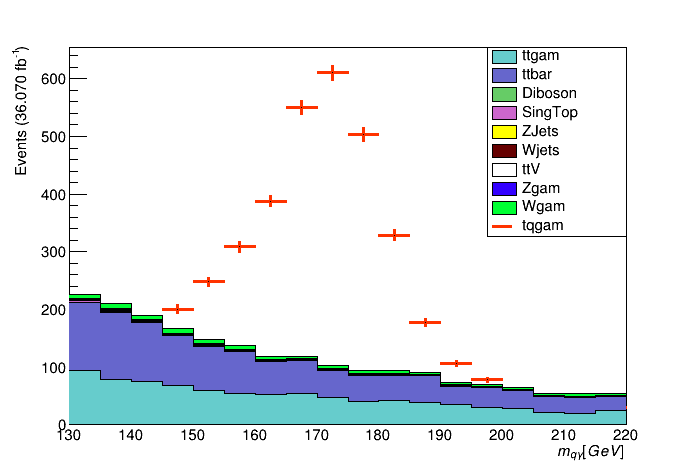
\includegraphics[width=.9\textwidth]{../../ThesisImages/plotsloose/mu_h_qgam_m.png}
\end{column} 
\begin{column}{0.5\textwidth}
\begin{itemize}
\item After Cuts
\end{itemize}
\centering
\includegraphics[width=.9\textwidth]{../../ThesisImages/plotsstrict/el_h_qgam_m.png}\\
\includegraphics[width=.9\textwidth]{../../ThesisImages/plotsstrict/mu_h_qgam_m.png}
\end{column}
\end{columns}
}



%%%%%%%%%%%%%%%%%%%%%%%%%%%%%%%%%%%%%%%%%%%%%%%%%%%%%%%%%%%%%%%%%%
\section{}
\subsection{Outlook}
\frame{\frametitle{Outlook}
\begin{itemize}
\item Many improvements can be made to the analysis
\begin{itemize}
\item Investigation of $\chi^2$ as a discriminating variable
\item Inclusion of isolation and spatial proximity cuts
\end{itemize}
\item Monte Carlo distributions can be used to set an expected limit on the Branching Ratio
\end{itemize}
\centering
\includegraphics[width=.5\textwidth]{../../ThesisImages/plotsstrict/el_h_min_chi2.png}
\captionof{figure}{e-channel $\chi^2$ after Z, Bjet cuts}
}


\subsection{Conclusion}
\frame{\frametitle{Conclusion}
\begin{itemize}
\item An excess signal would be indicative of some physics beyond the Standard Mode that couples strongly to the top sector
\item The search for FCNCs with enhanced rates are important pieces of testing many new theories
\item The LHC continues to produce copious data to look though for these events!
\item Barring any excess: with $\approx 150 \text{fb}^{-1}$ data at $\sqrt{s}=$ 13TeV setting an upper limit of  $\text{BR}(t\rightarrow q \gamma) <  3x10^{-5}$ is a reasonable goal, extrapolating from past results. 
\end{itemize}
}


%%%%%%%%%%%%%%%%%%%%%%%%%%%%%%%%%%%%%%%%%%%%%%%%%%%%%%%%%%%%%%%%

\appendix
\section{Backup}
\frame{\frametitle{Backup}
}
\frame{\frametitle{Integrated Luminosity}
\centering
\includegraphics[width=1.\textwidth]{../../ThesisImages/2017PeakLumiByFill.pdf}
}
\frame{\frametitle{A Couple BSM Diagrams}
\centering
\includegraphics[width=1.\textwidth]{../../ThesisImages/BSMDiagrams.png}
}

\frame{\frametitle{Jets/AntiKT}

\[ d_{ij} = min(\frac{1}{p_{ti}^2},\frac{1}{p_{tj}^2}) \frac{\Delta_{ij}^2}{R^2}
\]
\[ d_{iB} = \frac{1}{p_{ti}^2}
\]
\[ \Delta_{ij}^2 = (\eta_i -\eta_j )^2 + (\phi_i - \phi_j )^2
\]
\begin{itemize}
\item Find minimum of entire set of $\{ d_{ij},d_{iB} \}$
\item If $d_{ij}$ is the minimum particles i,j are combined into one particle and removed from the list of particles
\item If $d_{iB}$ is the minimum i is labelled as a final jet and removed from the list of particles
\item Repeat until all particles are part of a jet with distance between jet axes $\Delta_{ij}$ is greater than R
\end{itemize}
}

\frame{\frametitle{B-tagging}
\centering
\includegraphics[height=.8\textheight]{../../ThesisImages/B-tagging_diagram.png}

}
\frame{\frametitle{}
\[ \mathcal{L}^{eff}_{tq\gamma} = - e \bar{c} \frac{i \sigma^{\mu\nu}q_{\nu}}{m_t}(\lambda^{L}_{ct}P_L + \lambda^{R}_{ct}P_{R}) t A_{\mu} +H.c.
\]
}

\end{document}

%36.070
